%%%%%%%%%%%%%%%%%%%%%%%%%%%%%%%%%%%%%%%%%%%%%%%%%%%%%%%%%%%%%%%%%%%%
%% I, the copyright holder of this work, release this work into the
%% public domain. This applies worldwide. In some countries this may
%% not be legally possible; if so: I grant anyone the right to use
%% this work for any purpose, without any conditions, unless such
%% conditions are required by law.
%%%%%%%%%%%%%%%%%%%%%%%%%%%%%%%%%%%%%%%%%%%%%%%%%%%%%%%%%%%%%%%%%%%%

\documentclass[
  digital,     %% The `digital` option enables the default options for the
               %% digital version of a document. Replace with `printed`
               %% to enable the default options for the printed version
               %% of a document.
%%  color,       %% Uncomment these lines (by removing the %% at the
%%               %% beginning) to use color in the printed version of your
%%               %% document
  oneside,     %% The `oneside` option enables one-sided typesetting,
               %% which is preferred if you are only going to submit a
               %% digital version of your thesis. Replace with `twoside`
               %% for double-sided typesetting if you are planning to
               %% also print your thesis. For double-sided typesetting,
               %% use at least 120 g/m² paper to prevent show-through.
  nosansbold,  %% The `nosansbold` option prevents the use of the
               %% sans-serif type face for bold text. Replace with
               %% `sansbold` to use sans-serif type face for bold text.
  nocolorbold, %% The `nocolorbold` option disables the usage of the
               %% blue color for bold text, instead using black. Replace
               %% with `colorbold` to use blue for bold text.
  lof,         %% The `lof` option prints the List of Figures. Replace
               %% with `nolof` to hide the List of Figures.
  nolot,         %% The `lot` option prints the List of Tables. Replace
               %% with `nolot` to hide the List of Tables.
]{fithesis4}
%% The following section sets up the locales used in the thesis.
\usepackage[resetfonts]{cmap} %% We need to load the T2A font encoding
\usepackage[T1,T2A]{fontenc}  %% to use the Cyrillic fonts with Russian texts.
\usepackage[
  main=english, %% By using `czech` or `slovak` as the main locale
                %% instead of `english`, you can typeset the thesis
                %% in either Czech or Slovak, respectively.
  english, german, czech, slovak %% The additional keys allow
]{babel}        %% foreign texts to be typeset as follows:
%%
%%   \begin{otherlanguage}{german}  ... \end{otherlanguage}
%%   \begin{otherlanguage}{czech}   ... \end{otherlanguage}
%%   \begin{otherlanguage}{slovak}  ... \end{otherlanguage}
%%
%%
%% The following section sets up the metadata of the thesis.
\thesissetup{
    date        = \the\year/\the\month/\the\day,
    university  = mu,
    faculty     = fi,
    type        = mgr,
    department  = Department of Computer Systems and Communications,
    author      = Bc. Pavol Baran,
    gender      = m,
    advisor     = {RNDr. Lukáš Hejtmánek, Ph.D.},
    title       = {Checkpoint/Restore in Jupyterhub},
    TeXtitle    = {Checkpoint/Restore in Jupyterhub},
    keywords    = {JupyterHub, JupyterLab, Jupyter Notebook, Kubernetes, Checkpoint, Restore, Spawner},
    TeXkeywords = {JupyterHub, JupyterLab, Jupyter Notebook, Kubernetes, Checkpoint, Restore, Spawner},
    abstract    = {TODO: at the end},
    thanks      = {I would like to thank my advisor RNDr. Lukáš Hejtmánek, Ph.D., for his help and guidance, as well as RNDr. Viktória Spišaková for helping me troubleshoot CRIU issues. Lastly, I want to thank my family and friends for supporting me throughout this tough period of my life.},
    bib         = example.bib,
    %% Remove the following line to use the JVS 2018 faculty logo.
    facultyLogo = fithesis-fi,
}
\usepackage{makeidx}      %% The `makeidx` package contains
\makeindex                %% helper commands for index typesetting.
%% These additional packages are used within the document:
\usepackage{paralist} %% Compact list environments
\usepackage{amsmath}  %% Mathematics
\usepackage{amsthm}
\usepackage{amsfonts}
\usepackage{url}      %% Hyperlinks
\usepackage{markdown} %% Lightweight markup
\usepackage{listings} %% Source code highlighting
\lstset{
  basicstyle      = \ttfamily,
  identifierstyle = \color{black},
  keywordstyle    = \color{blue},
  keywordstyle    = {[2]\color{cyan}},
  keywordstyle    = {[3]\color{olive}},
  stringstyle     = \color{teal},
  commentstyle    = \itshape\color{magenta},
  breaklines      = true,
}
\usepackage{floatrow} %% Putting captions above tables
\floatsetup[table]{capposition=top}
\usepackage[babel]{csquotes} %% Context-sensitive quotation marks

%%Does \Cref links
\usepackage{hyperref}
\usepackage{cleveref}

% Only 2 leveled Contents
\addtocontents{toc}{\setcounter{tocdepth}{1}}


% CODE LISTING
\lstdefinelanguage{Go}{
  % Keywords as defined in the language grammar
  morekeywords=[1]{%
    break,default,func,interface,select,case,defer,go,map,%
    struct,chan,else,goto,package,switch,const,fallthrough,%
    if,range,type, continue,for,import,return,var},
  % Built-in functions
  morekeywords=[2]{%
    append,cap,close,complex,copy,delete,imag,%
    len,make,new,panic,print,println,real,recover},
  % Pre-declared types
  morekeywords=[3]{%
    bool,byte,complex64,complex128,error,float32,float64,%
    int,int8,int16,int32,int64,rune,string,%
    uint,uint8,uint16,uint32,uint64,uintptr},
  % Constants and zero value
  morekeywords=[4]{true,false,iota,nil},
  % Strings : "foo", 'bar', `baz`
  morestring=[b]{"},
  morestring=[b]{'},
  morestring=[b]{`},
  % Comments : /* comment */ and // comment
  comment=[l]{//},
  morecomment=[s]{/*}{*/},
  % Options
  sensitive=true
}
\lstset{language=Go,
  basicstyle=\ttfamily\scriptsize,
  keywordstyle=\color{blue}\ttfamily,
  stringstyle=\color{red}\ttfamily,
  commentstyle=\color{green}\ttfamily}

% END CODE


\usepackage[newfloat]{minted}
\usepackage{caption}
\newenvironment{code}{\captionsetup{type=listing}}{}
\SetupFloatingEnvironment{listing}{name=Listing}



\begin{document}
%% The \chapter* command can be used to produce unnumbered chapters:
\chapter*{Introduction}
%% Unlike \chapter, \chapter* does not update the headings and does not
%% enter the chapter to the table of contents. I we want correct
%% headings and a table of contents entry, we must add them manually:
\markright{\textsc{Introduction}}
\addcontentsline{toc}{chapter}{Introduction}

TODO: at the end approx 1 page

\chapter{Project Jupyter}
As this thesis focuses on checkpointing and restoring Jupyter Notebooks within JupyterHub, it begs the question: what even is JupyterHub or Jupyter Notebook? The first part of this chapter provides a brief look into what Jupyter Notebook is and how it is used before examining its next-generation successor, JupyterLab. The second part discusses JupyterHub, deconstructs it into its fundamental pieces, and describes each piece in detail to give a solid foundation of the inner workings of JupyterHub. The last part describes the specific distribution of JupyterHub on which this thesis builds.

Jupyter Notebook, JupyterLab, and JupyterHub all share one thing in common: their umbrella project, Jupyter.
\emph{Project Jupyter is an open-source software project and community that builds software, services, and open standards for interactive computing across dozens of programming languages} \cite{granger2021jupyter}.
Project Jupyter and Jupyter originated from the IPython project, which provided an improved interactive Python shell over the default one \cite{ipython}. The same IPython now serves as the default execution engine (\emph{Kernel}) for Jupyter Notebook.

Nowadays, Jupyter Notebooks are widely used in data science, machine learning, and scientific research for tasks like data analysis, with over ten million notebook documents available on GitHub \cite{granger2021jupyter}. In scientific research, Jupyter Notebooks allow researchers to document experiments, perform simulations, and share reproducible procedures. Educators use Jupyter Notebooks for interactive teaching, enabling students to simultaneously learn programming, mathematics, and data visualization. 
Finally, businesses use it to create dashboards and reports, helping them organize and communicate data to support informed decisions.

\section{Jupyter Notebook}
Jupyter Notebook is an open-source application that allows users to easily create and share computational notebooks - documents that combine code, interactive controls, plain language, graphs, and figures, among other visualizations \cite{granger2021jupyter}. Although there exist other projects focused on computation notebooks, such as the proprietary Wolfram Mathematica\footnote{\url{https://www.wolfram.com/mathematica/}}, Jupyter Notebooks gained widespread adoption due to its open-source nature and simplicity.

The ability to create a computational notebook comes from the fact that Jupyter Notebook runs as a web server, providing its user interface in a web browser, through which users can write code with auto-completion, execute the code, as well as provide descriptions or annotate the code using Markdown or LaTeX languages. On the other hand, the ability to share computational notebooks stems from the simple format in which the notebooks are stored \cite{jupyter_notebook}.

\begin{figure}[H]
  \begin{center}
  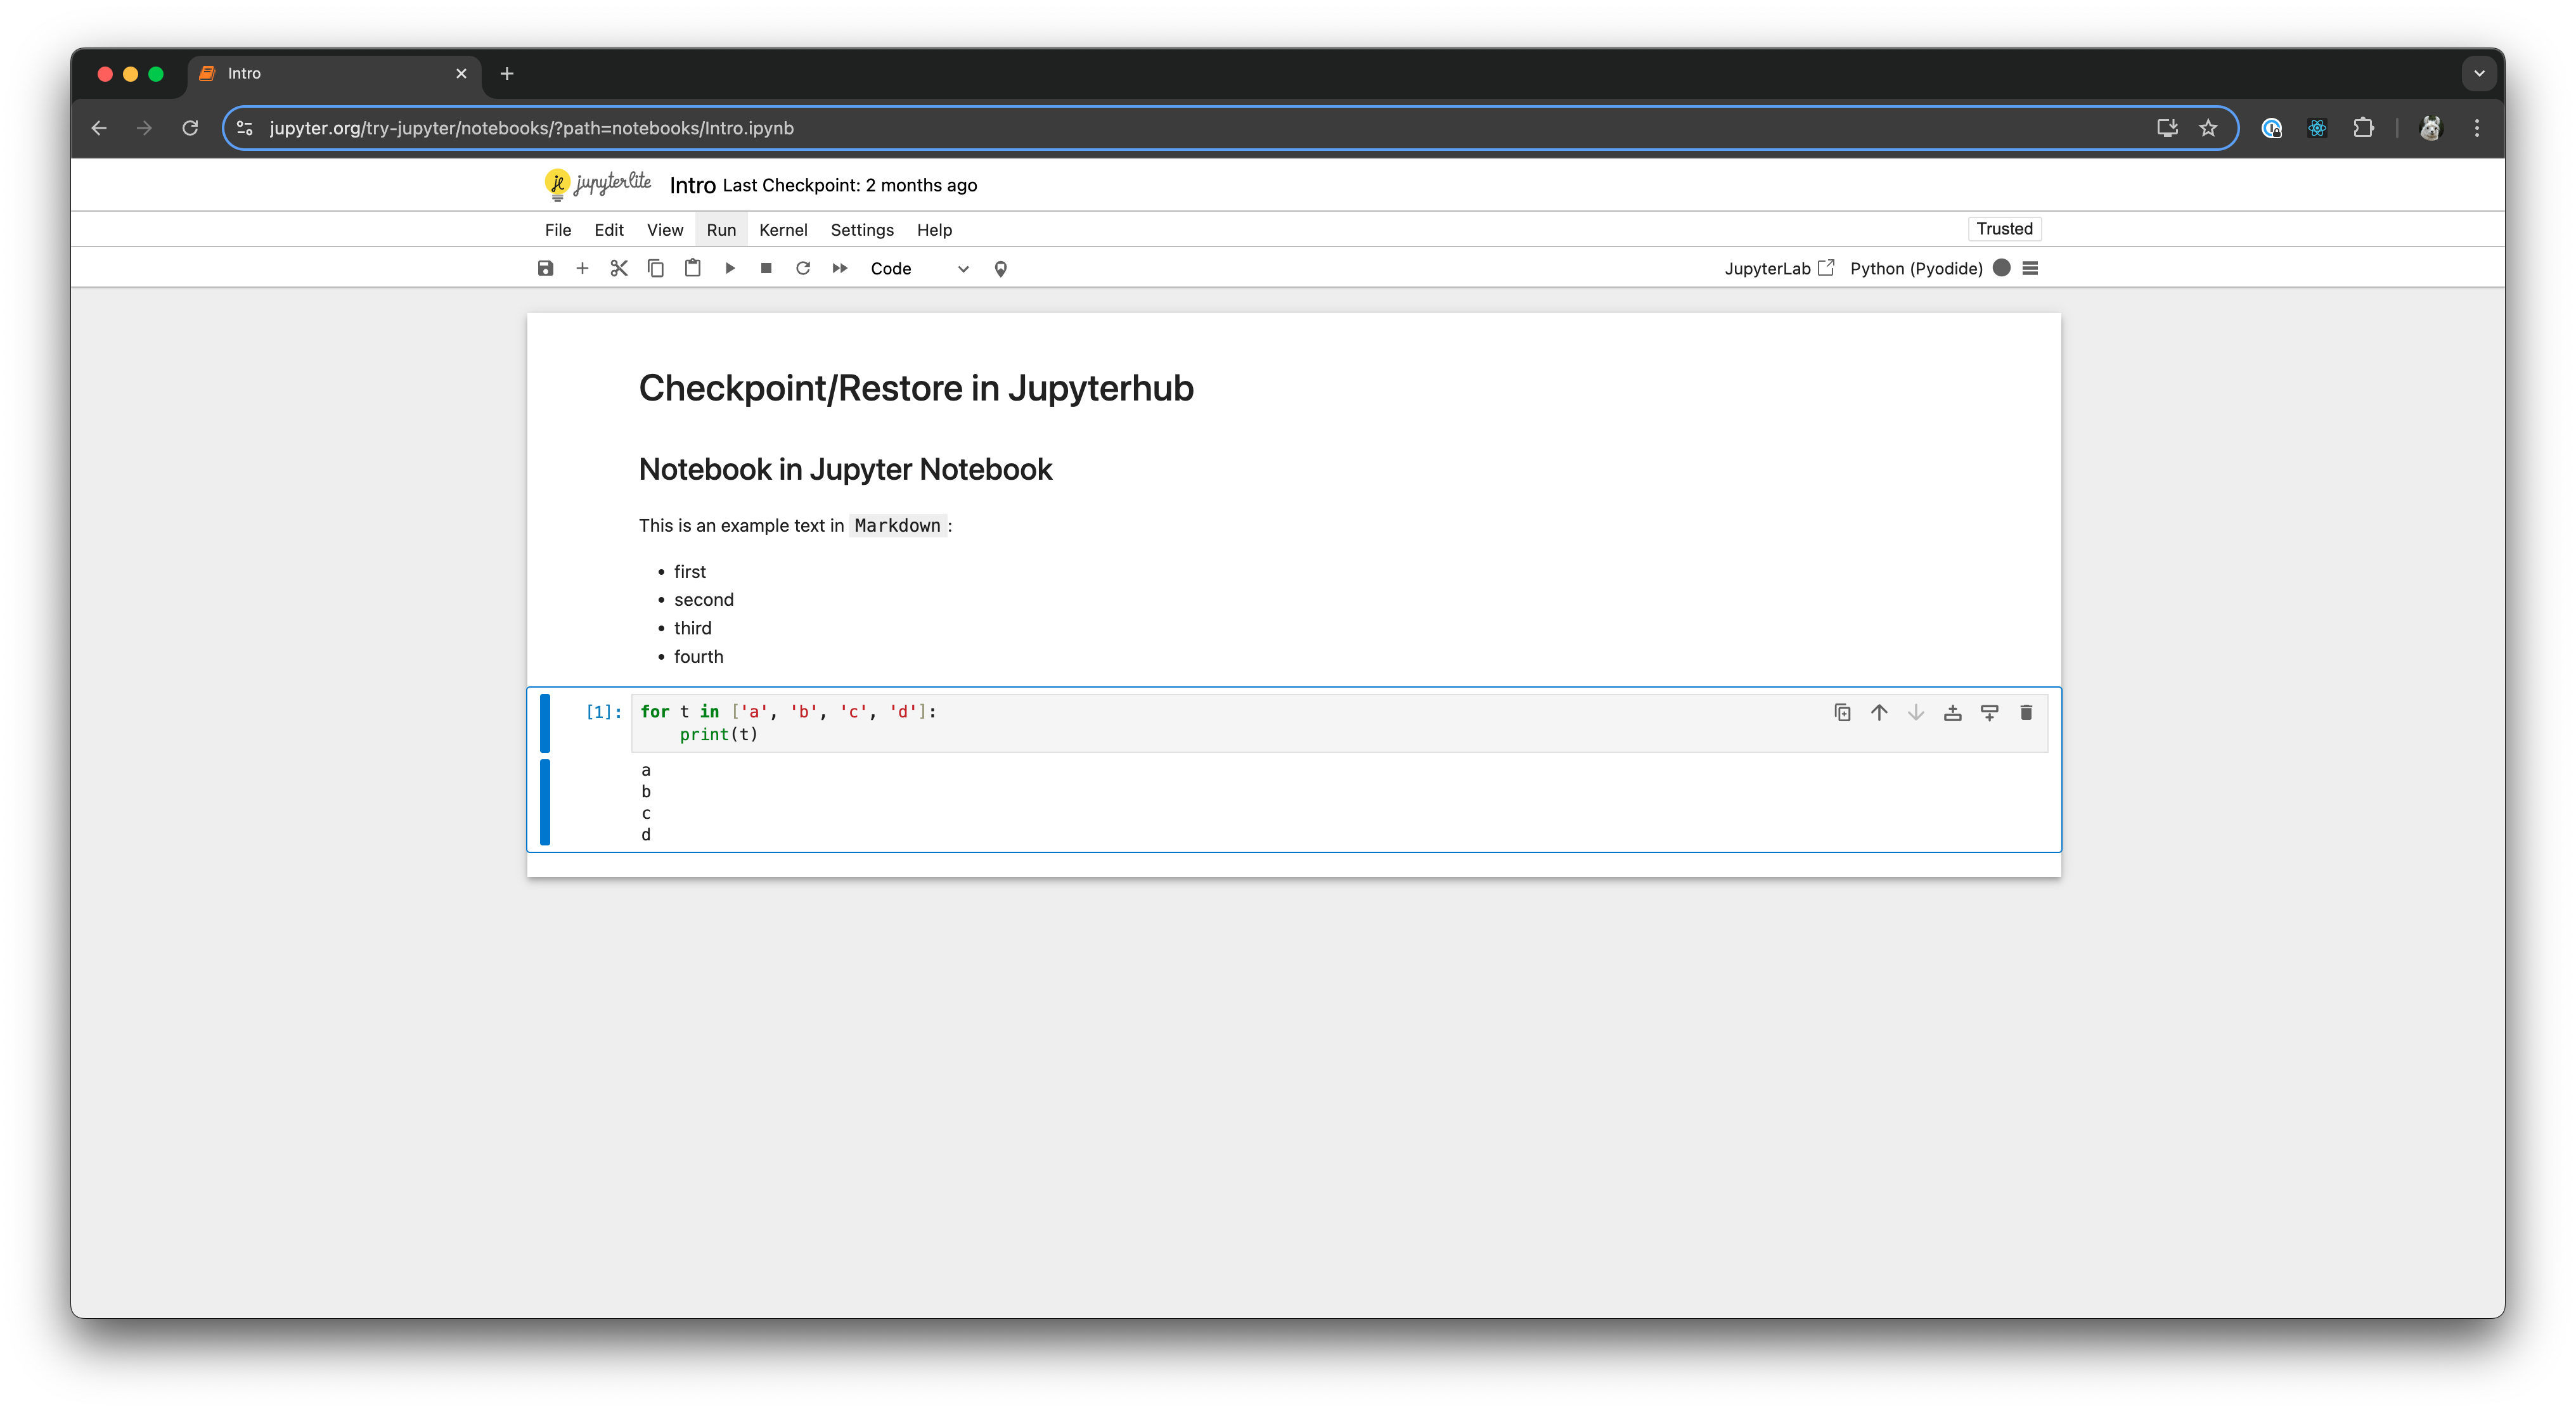
\includegraphics[width=\textwidth]{figures/jupyter-notebook-screenshot.png}
  \end{center}
  \caption{Jupyter Notebook's user interface.}
  \label{fig:jupyter-notebook-screenshot}
\end{figure}

\Cref{fig:jupyter-notebook-screenshot} shows the Notebook's user interface (UI) accessible through a standard web browser. The UI provides common keyboard shortcuts for editing and, as already mentioned, auto-completion of code. However, apart from the functionality of any word processor, the UI allows for the manipulation of cells. These cells are the main building blocks of the notebook document, and there are three types of cells, each serving a specific purpose in structuring the notebook document:

\begin{description}

    \item[Code cell]
    These cells allow for writing and executing code in a particular language, the most common being Python. The actual type of language depends on the \emph{Kernel} with which the Jupyter Notebook server is communicating. The exact mechanism behind the execution of code in the Notebook is out of the scope of this thesis. Nevertheless, there are Kernels for \emph{dozens} of languages, letting users choose from \emph{over a hundred} \cite{perkel2018jupyter} different Kernels.

    \item[Markdown cell]
    These cells are meant for any text describing, explaining, or commenting on the code. Generally, the text in these cells is in Markdown language. However, mathematical notations can also be prescribed using LaTeX \cite{jupyter_notebook}. 
    
    \item[Raw cell]
    Unlike Markdown and Code cells, text in raw cells will be uninterpreted by Jupyter Notebook. Raw cells preserve the content exactly as it is written, which makes them practical in including plain text, scripts in other languages, or data in a specific format that should not alter the notebook's environment.
    
\end{description}

The notebook documents, also commonly referred to as Jupyter Notebooks, or just notebooks 
\footnote{Throughout this thesis, the name \emph{Jupyter Notebook}, will reference only the application itself, not the notebook document that can be created within the application.}
are stored in an open document format based on JSON, with the file itself using \emph{.ipynb} extension. The document contains a complete record of the user's sessions, including the output of the executed code. Since JSON is a plain text format, it allows for version control using Git and easy conversion to other formats, such as HTML, LaTeX, or PDF, using the included tool \emph{nbconvert}. The authors can publish their notebooks to GitHub, share the notebook as an HTML page online, or print the PDF on paper and share it physically \cite{kluyver2016jupyter}. 

% Maybe TODO: Jupyter Notebook has become widely used in AI research communities \url{ https://cdn.aaai.org/ocs/10349/10349-46093-1-PB.pdf} and other academical environments with over milion \url{https://ieeexplore.ieee.org/abstract/document/8816763} notebooks available online.

\section{JupyterLab}

JupyterLab's documentation describes JupyterLab as Jupyter Notebook's \emph{sibling} \cite{jupyter_lab}. However, referring to it as a sibling might give the impression that JupyterLab is merely an alternative to Jupyter Notebook. In reality, JupyterLab represents a significant advancement, offering a more sophisticated and customizable user interface that can be tailored to different use cases. JupyterLab retains the core functionalities of Jupyter Notebook, one of which is the document format. However, it expands significantly upon them by providing a modular, flexible workspace that supports multiple panels and interactive widgets, as seen on \Cref{fig:jupyter-lab-screenshot}. Whereas Jupyter Notebook's user interface (\Cref{fig:jupyter-notebook-screenshot}) centers around one notebook document, JupyterLab resembles more of an integrated development environment (IDE), with file browser on the hand left side and a variable inspector on the right.

\begin{figure}[H]
  \begin{center}
  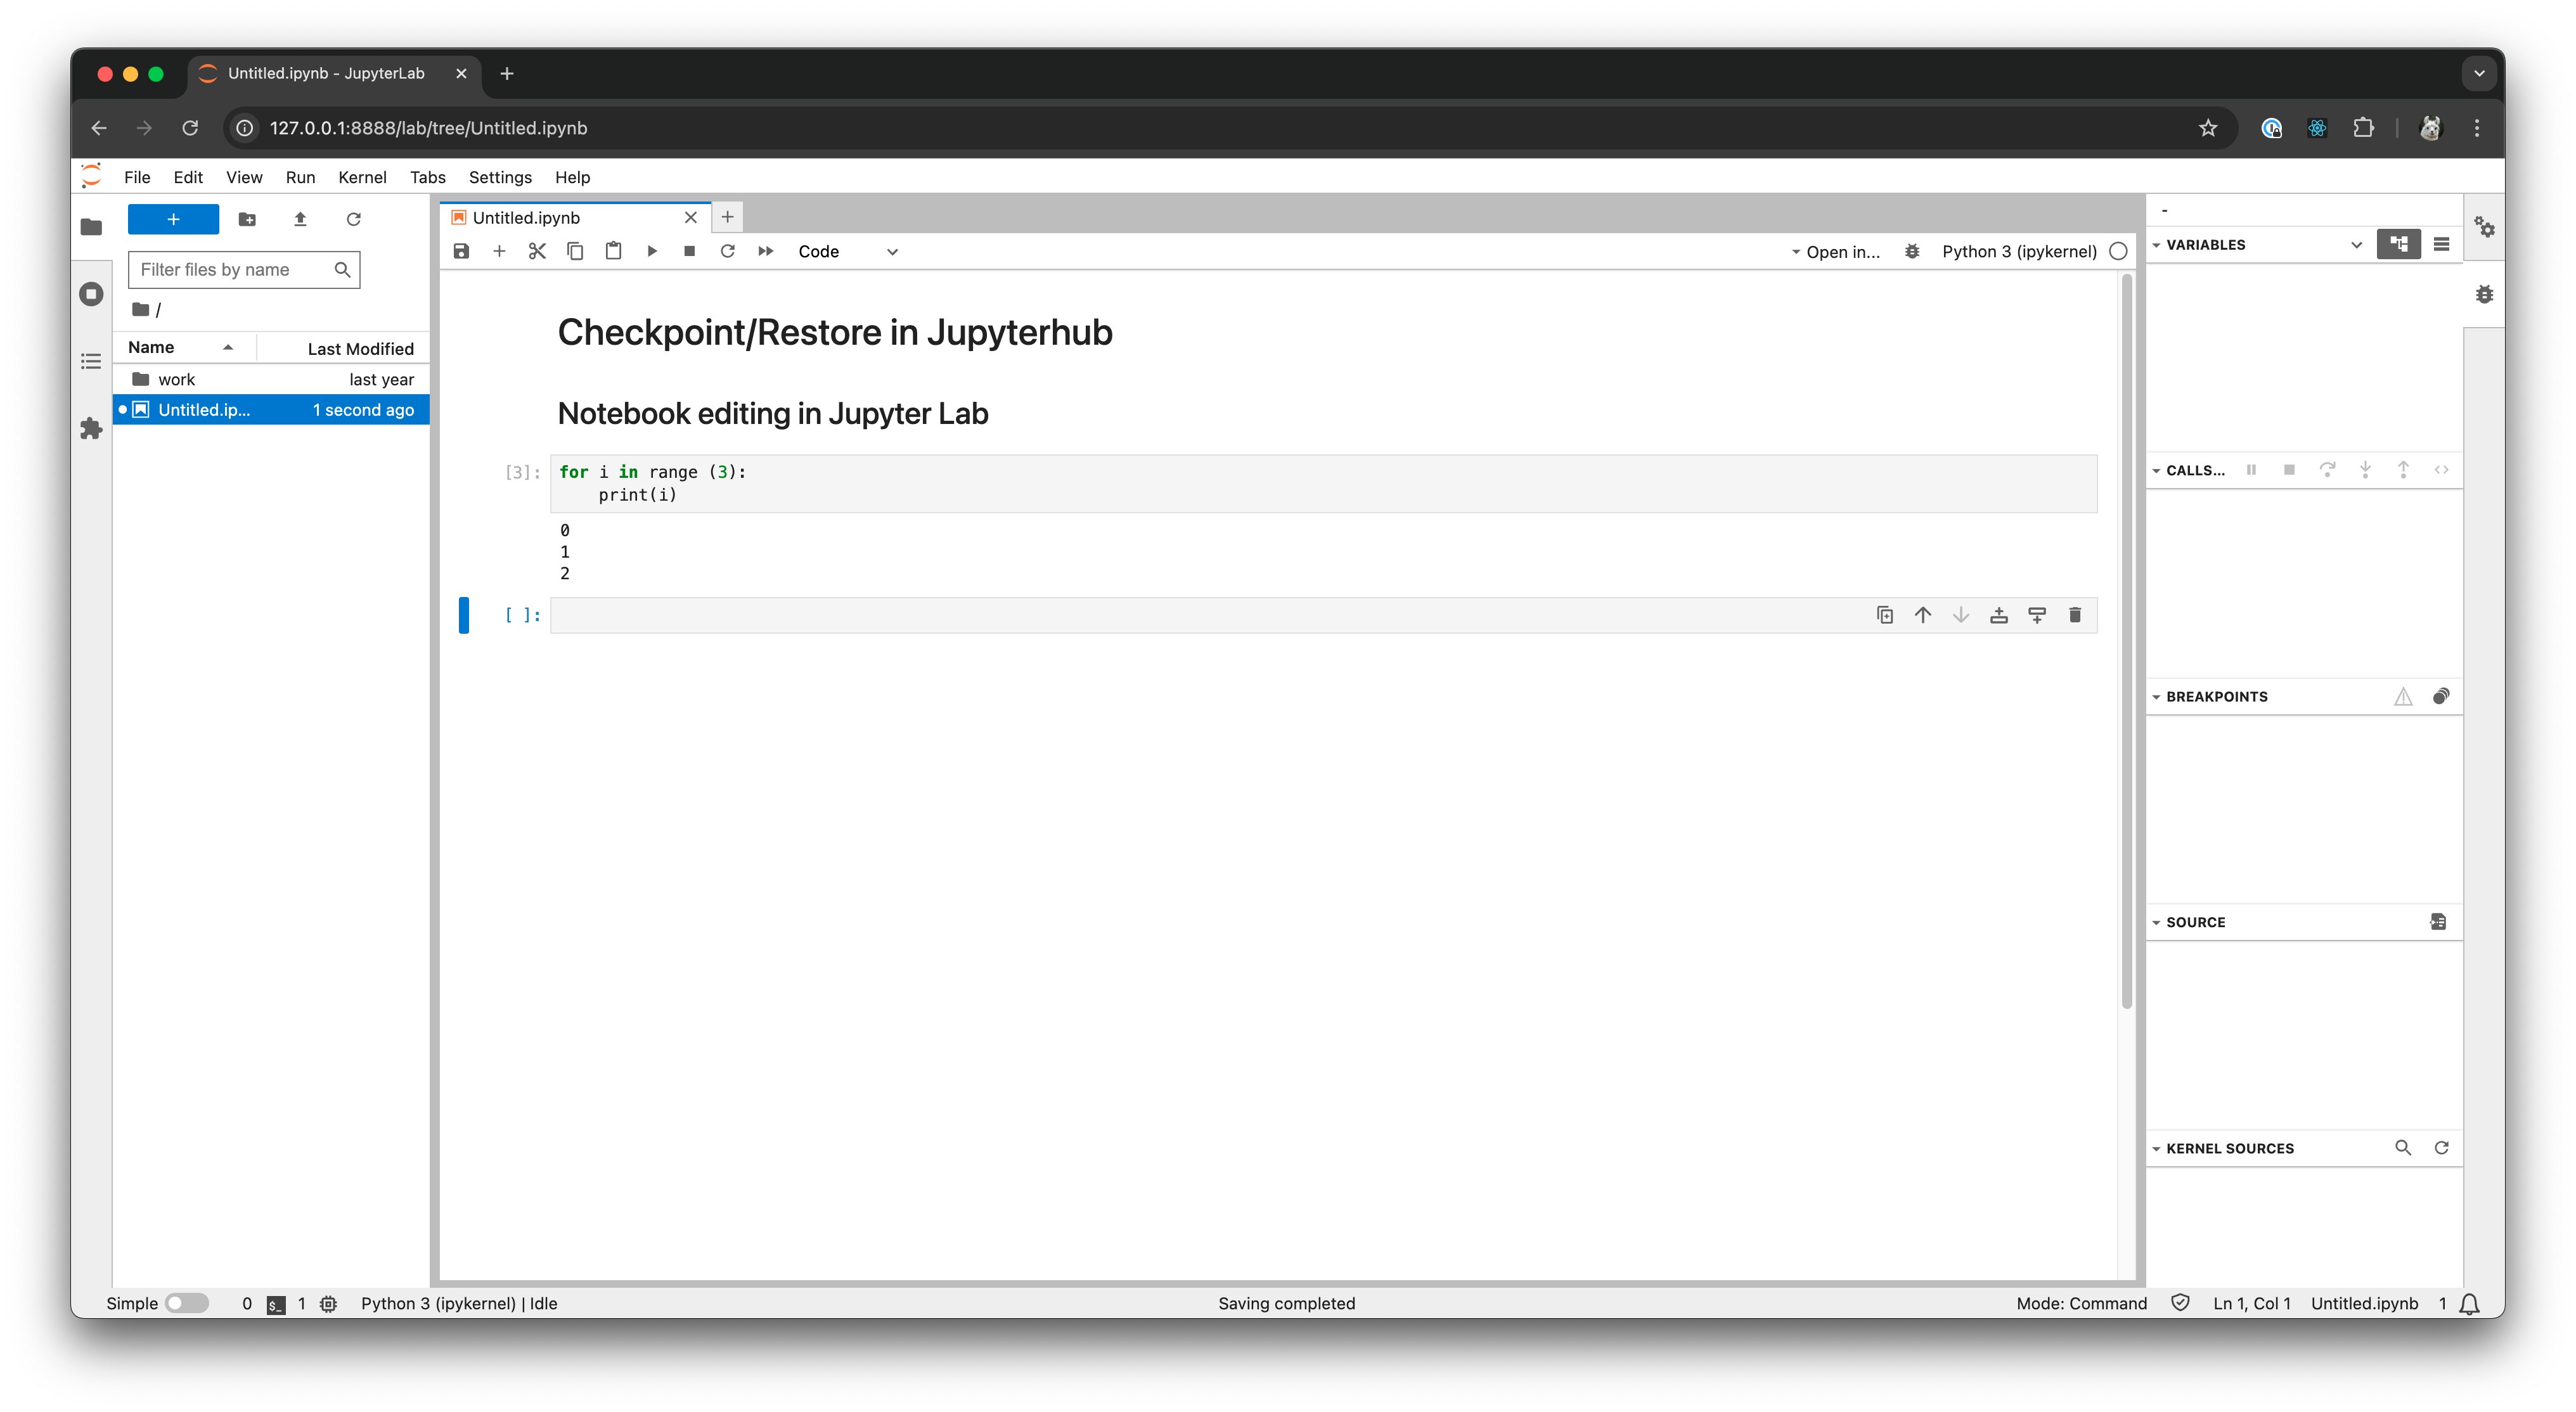
\includegraphics[width=\textwidth]{figures/jupyter-lab-extended-screenshot.png}
  \end{center}
  \caption{JupyterLab's user interface.}
  \label{fig:jupyter-lab-screenshot}
\end{figure}

All this does not negate the fact that some individuals still prefer the comparably simplified interface of Jupyter Notebook or do not see the value in upgrading. Moreover, as JupyterLab supports the same \emph{.ipynb} document format, and the initial versions depended on the installation of Notebook; it is not uncommon, in the community and documentation, to refer to JupyterLab as Jupyter Notebook instead. Consequently, since JupyterHub (\Cref{sec:jupyterhub}) supports both JupyterLab and Jupyter Notebook, this thesis will, henceforth, adopt the term Jupyter Notebook exclusively.

\section{JupyterHub}
\label{sec:jupyterhub}
Jupyter Notebook was initially designed for single-user environments. However, as Jupyter Notebook's popularity rose among researchers, data analysts, and academics, such did the need for a way to quickly deploy Jupyter Notebooks for multiple users in a centralized environment without requiring each user to install Jupyter Notebook. In other words, \emph{IT support for 800 students, helping them debug why the installation on their laptop is not working; that's simply infeasible} \cite{perkel2018jupyter}.

JupyterHub addressed this need by providing a \emph{multi-user Hub that creates, manages, and proxies multiple instances of the single-user Jupyter notebook server}, which allows it to be used in \emph{a class of students, a corporate data science group, or a scientific research group} \cite{jupyterhub}. Simply put, JupyterHub takes the single-user Jupyter Notebook and adds a layer of functionality on top, providing user management and control over the running environment of the Notebooks.

To account for different use cases, serving Jupyter Notebooks to a few as well as hundreds and thousands of users, JupyterHub comes in two distinct distributions:
\begin{description}

    \item[The Littlest JupyterHub (TLJH)]
    Intended primarily for educators teaching small classes of ten to at most a hundred students. The distribution runs on a single server without any containerization technology such as Docker or Kubernetes and intends to provide as simple as possible installation and configuration setup for JupyterHub \cite{littlest_jupyterhub}.

    \item[Zero to JupyterHub with Kubernetes (Z2JH)]
    This distribution runs in Kubernetes, with many of its components running in separate containers, which allow it to dynamically scale up or down depending on the required resources and user demand. By utilizing several Kubernetes Nodes, the distribution can serve even a thousand users \cite{jupyterhub}. This thesis builds upon Z2JH; therefore, \Cref{sec:z2jh} provides a more detailed look into this distribution.
    
\end{description}

Although using one of the distributions gives some assurance of scalability, it is not the only way to run JupyterHub. JupyterHub can be run as any Python application and configured to use specific \emph{Authenticator, Spawner, and Services} (see \Cref{subsec:jupyterhub:architecture}) based on a particular use-case needed to fulfill. The unofficial distribution, \emph{JupyterHub the hard way}\footnote{\url{https://github.com/jupyterhub/jupyterhub-the-hard-way/blob/master/docs/installation-guide-hard.md}}, provides a thorough walk-through for setting up JupyterHub from scratch.


\section{JupyterHub's Architecture}
\label{subsec:jupyterhub:architecture}
JupyterHub comprises several subsystems as depicted on \Cref{fig:jupyter-hub-arch}, many of which have multiple implementations, enabling administrators to pick and choose the best fit for their specific use case, such as different Spawners, Authenticators, and Services. The following subsections provide a brief look into the most significant components.

\begin{figure}[H]
  \begin{center}
  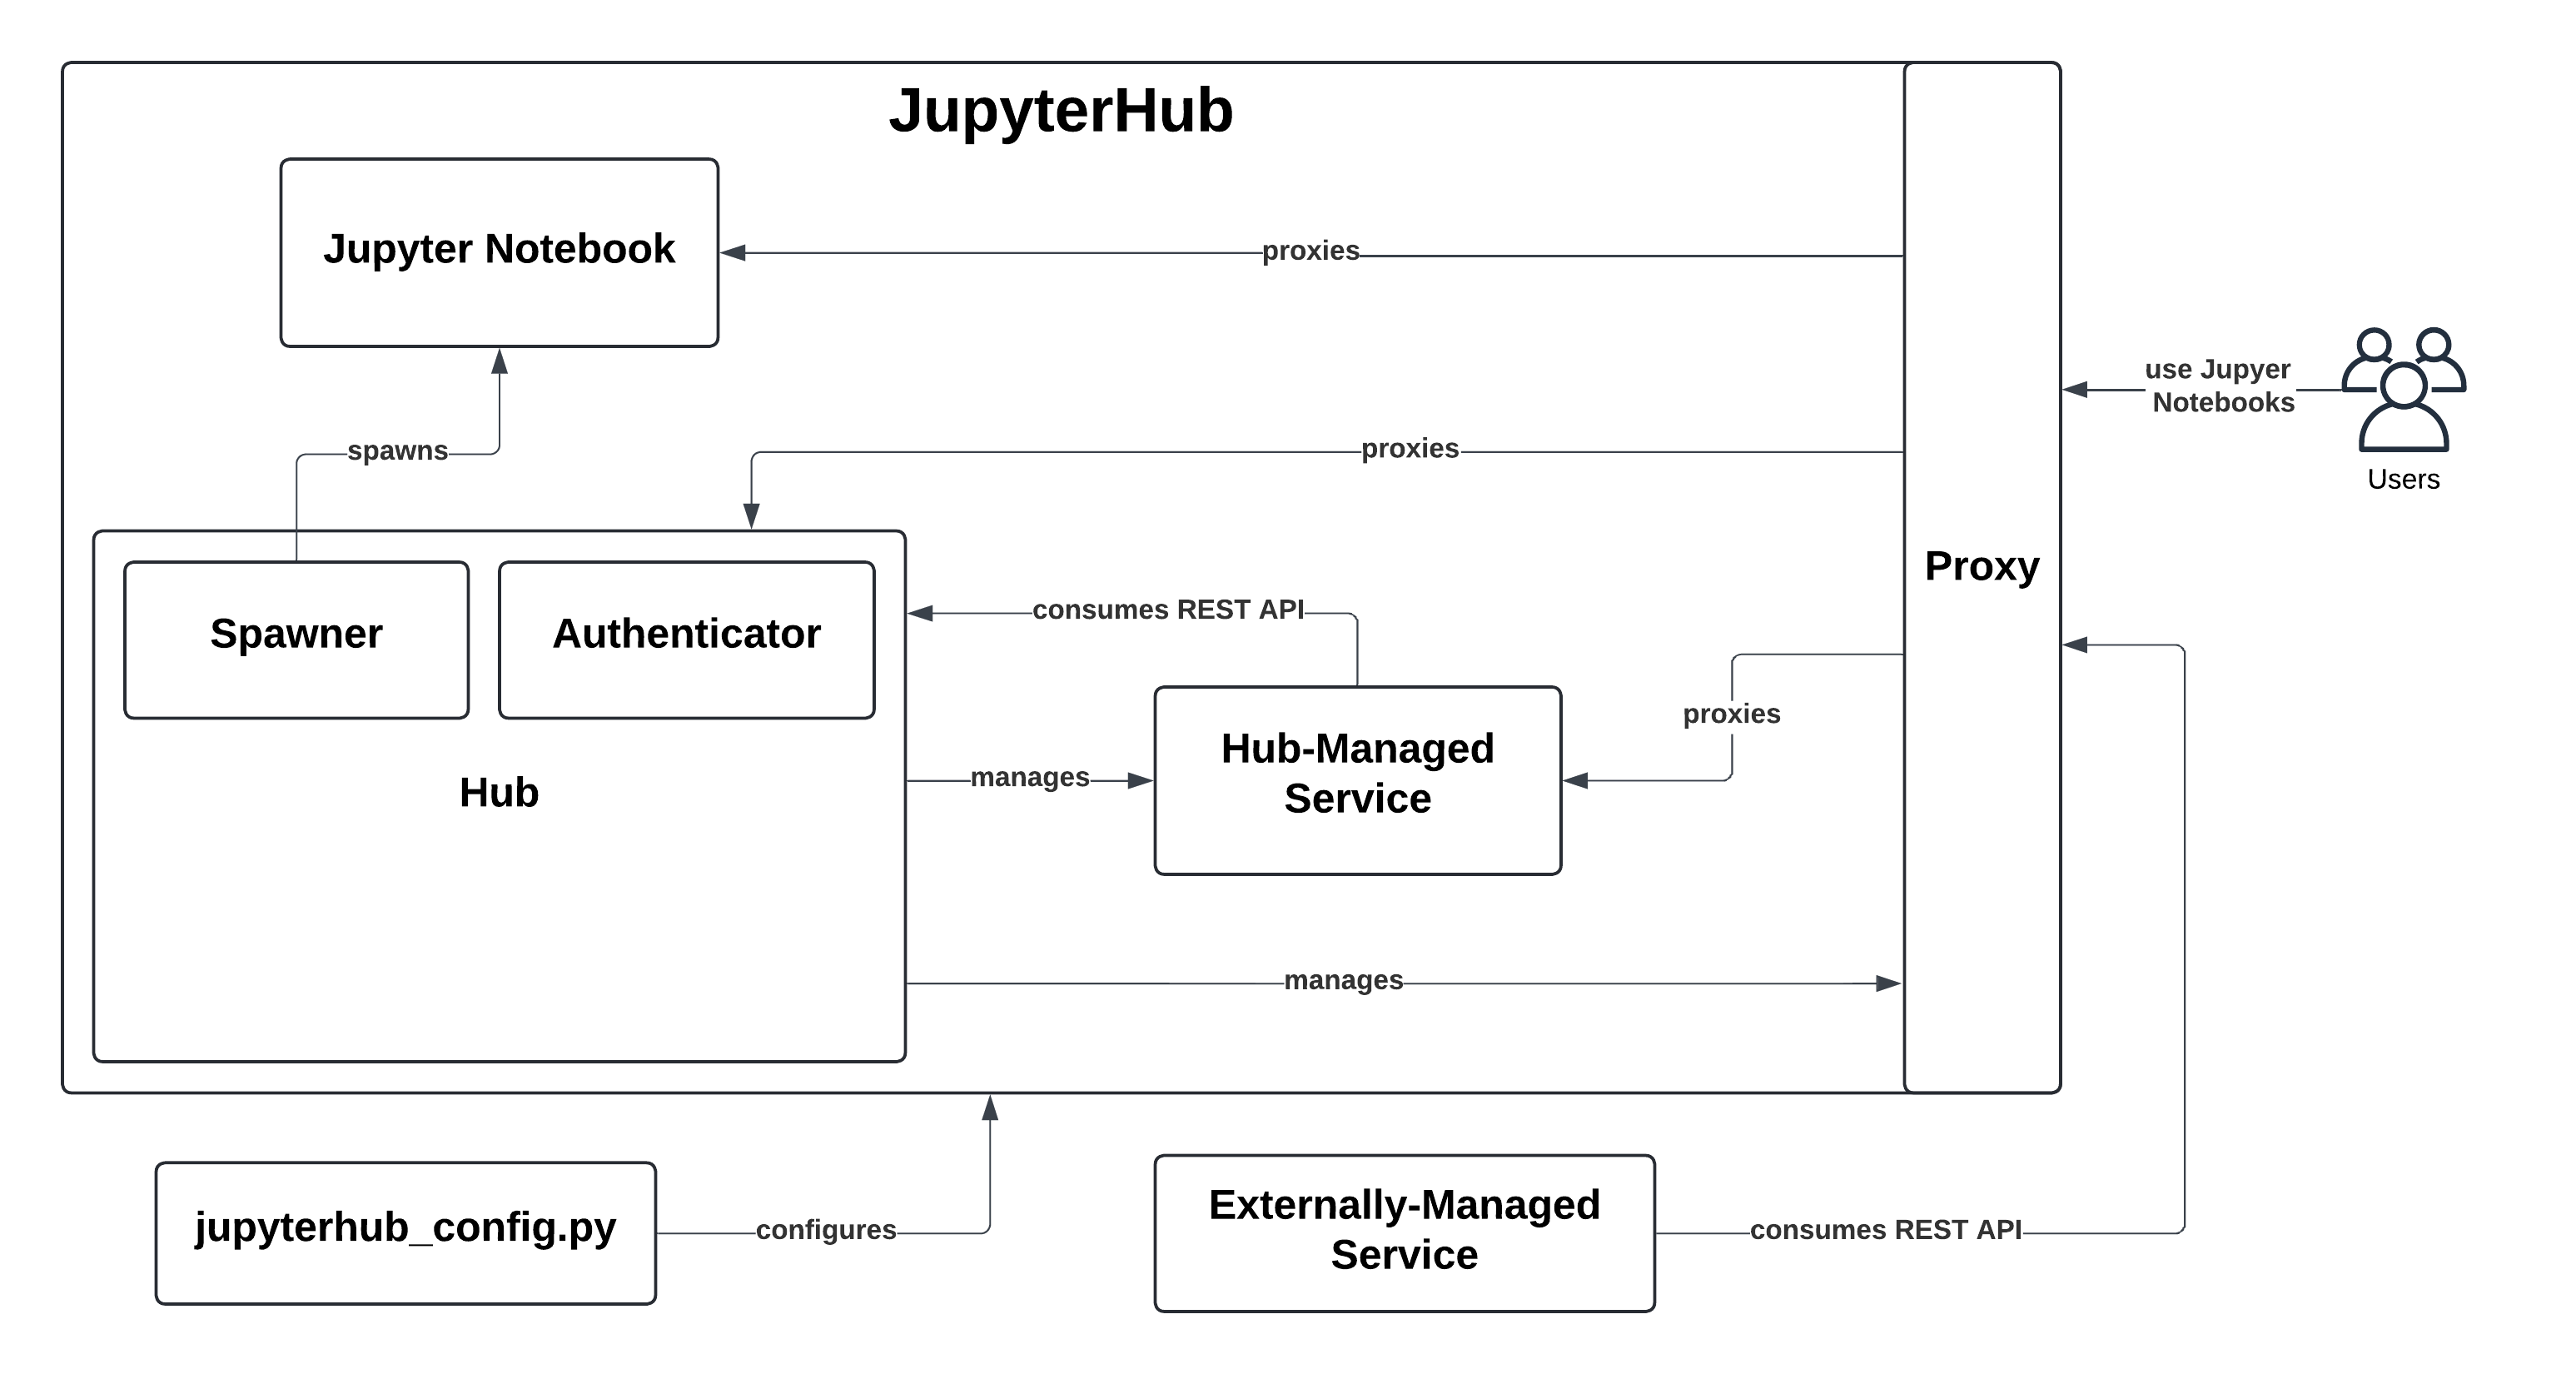
\includegraphics[width=\textwidth]{figures/jupyer-hub-architecture.png}
  \end{center}
  \caption{Architecture of JupyterHub. }
  \label{fig:jupyter-hub-arch}
\end{figure}

\subsection{Hub}
Hub is the central piece connecting all the components. Nevertheless, the end-user only interacts with Hub briefly during login authentication and initialization or shutdown of Jupyter Notebooks. Hub's role is orchestrational in that it starts and stops the Proxy and Services processes, instructs Spawner when to spawn or remove Notebooks, keeps track of users, and delegates authentication of users to the Authenticator.

\subsection{Proxy}
The Proxy, specifically reverse Proxy, serves as an ingress to JupyterHub. Each connection to JupyterHub and, thereby, to the spawned Notebooks goes through the Proxy. This implies that both the Hub and all Notebook applications have to be reachable by the Proxy\cite{jupyterhub_arch}.

When a user connects to JupyterHub for the first time, the Proxy forwards the connection to the Hub. Hub then delegates user authentication to the Authenticator, and only when the user is authenticated does the Hub instruct the Spawner to spawn the Jupyter Notebook. Once the Notebook is up and running, the Hub will update the routing table in the Proxy to forward connections from the specific user\footnote{user's session is tracked using a cookie.} to the spawned Notebook. Afterward, the Proxy forwards each connection of this specific user directly to the Notebook until the user's credentials expire and the whole flow is repeated, except if the Notebook is already running, it does not need to be spawned again.

Hub will start the Proxy as a separate process and stop it on shutdown if it is not configured otherwise. The Proxy can be configured to run entirely separately. Such configuration would allow users to continue using their Notebooks for a certain time, even in case of Hub's unexpected termination \cite{jupyterhub_arch}.

\subsection{Authenticator}
\label{subsec:jupyterhub:authenticator}

Whenever Hub needs to authorize a user's connection or request, it delegates this task to the Authenticator. The Authenticator serves as an interface between Hub and a user management system, allowing validation of user credentials and management of user accounts to be decoupled from JupyterHub. Specifically, Authenticator is part of Hub's codebase, a Python class that can be extended to provide desired functionality.

To keep track of which Notebook belongs to which user, among other tasks, the Hub has to record information about users in a database outside the Authenticator class. Even so, the Hub stores only the data relevant to the user's role and activities in JupyterHub and does not store the users themselves. The management of users, which users exist, and how users login is left up to the Authenticator \cite{jupyterhub_arch}.

Many Authenticator implementations available delegate the user management to a third-party identity provider through OAuth (OAuthenticator), LDAP (ldapauthenticator), or the PAMAuthenticator included in JupyterHub by default, which utilizes the PAM mechanism in Linux to authenticate users. One exception to that is the NativeAuthenticator, which, in fact, stores and validates its own usernames and passwords, effectively managing all users within JupyterHub only. The other exception is the DummyAuthenticator, which, mainly for testing purposes but not only, allows any user to log in \cite{jupyterhub_arch}.

\subsection{Spawner}
\label{sec:spawner}
Similar to how Authenticator is an interface between Hub and the user management system, the Spawner is an interface between Hub and the running environment of Notebooks. Like Authenticator, Spawner is a Python class in Hub's codebase and has multiple implementations deciding where and how Jupyter Notebooks should be spawned. 

To define itself as Spawner, the Python class needs to be able to perform three actions \cite{jupyterhub_spawner}:
\begin{itemize}
  \item start a Jupyter Notebook
  \item poll whether a Jupyter Notebook is still running
  \item stop a Jupyter Notebook
\end{itemize}
These actions map one-to-one to the class's \emph{start}, \emph{poll}, and \emph{stop} methods. Additionally, as it should be possible for the Hub to stop without affecting the Notebooks, the Spawner can take advantage of two methods, allowing it to persist its internal state across restarts. Hub will call the \emph{load\_state} method for a Spawner to restore its object properties from the state in the database, and \emph{get\_state} to get the internal state of the Spawner to be persisted \cite{jupyterhub_spawner}.

By default, JupyterHub uses the LocalProcessSpawner to spawn Notebooks as local processes, which, however, does not work on Windows. Fortunately, there are many other Spawner implementations, with the notable ones being:
\begin{description}

    \item[DockerSpawner] Capable of spawning Notebooks in Docker containers on the same machine or using DockerSwarm for spawning Notebooks on remote machines \cite{jupyterhub_spawner}. The Spawner can utilize Docker's API and limit the Notebook's allowed CPU and memory usage.
    
    \item[SystemdSpawner]
    Enables to spawn Notebooks using \emph{systemd} the \emph{system and service manager} \cite{systemd} for Linux. Similarly to DockerSpawner, it allows the CPU and memory to be limited for each Notebook. \textbf{The Littlest JupyterHub} distribution uses Spawner, which is based on SystemdSpawner.

    \item[SSHSpawner]
    Can be used to spawn Notebooks on a remote server through SSH. However, it seems that the repository of this Spawner\footnote{https://github.com/NERSC/sshspawner} is no longer actively maintained.

    \item[KubeSpawner]
    Allows spawning Notebooks as Kubernetes Pods and, therefore, can utilize the full potential of Kubernetes API, which implies that JupyterHub must be running in the Kubernetes cluster. This is the Spawner that the \textbf{Zero to JupyterHub with Kubernetes} distribution uses, and as such, this thesis is extending this Spawner with checkpoint and restore capabilities (\Cref{chap:checkpoint_spawner}).
    
\end{description}


\subsection{Services}
\label{subsec:jupyterhub:services}
Services are yet another way JupyterHub can be customized or extended. In the context of JupyterHub, a Service is defined \emph{as something (usually a process) that can interact with the Hub's REST API} \cite{jupyterhub_service}.

JupyterHub recognizes two types of Services. The first type, \textbf{Hub-Managed Service}, are services that are started as a sub-process of Hub and managed directly by Hub. The Hub takes responsibility for starting with a configured command and environment variables, stopping when requested or when the Hub stops, and restarting them when they unexpectedly terminate. The second type, \textbf{Externally-Managed Services}, are independent services that are not directly controlled by the Hub but still need to interact with it. In this case, the Service does not need to be a process; it might be any application. Both types of Services can be specified in JupyterHub's configuration file. However, only Externally-Managed Services can be added or removed at runtime \cite{jupyterhub_service}.

Adding a Service to JupyterHub can have three benefits. Firstly, the Service obtains an API token that it can use to call JupyterHub's REST API with configured permissions. The second benefit is that JupyterHub's Proxy can forward user requests to the Service, thus exposing the Service to the internet or other networks. Lastly, the Service can utilize Hub's authentication mechanism to be accessible only if the user's permissions allow him to.

\subsection{Configuration}
\label{subsec:jupyterhub:configuration}

To configure and customize all the components described, JupyterHub is set up to consume the traitlets\footnote{\url{https://github.com/ipython/traitlets}} configuration file, usually referred to as \emph{jupyterhub\_config.py}.

\begin{code}
\captionof{listing}{JupyterHub's configuration file jupyterhub\_config.py.}
\label{lst:jupyterhub:config}
\begin{minted}{yaml}
c.JupyterHub.ip = '0.0.0.0'
c.JupyterHub.port = 8000 
c.JupyterHub.authenticator_class = \ 
    'jupyterhub.auth.PAMAuthenticator'
c.JupyterHub.spawner_class = \
    'jupyterhub.spawner.LocalProcessSpawner'
\end{minted}
\end{code}

The \Cref{lst:jupyterhub:config} shows an example configuration of JupyterHub, setting the IP address and port the Proxy will listen on and specifying the implementation classes of Authenticator and Spawner.

\section{Zero to JupyterHub with Kubernetes}
\label{sec:z2jh}

Initial work on the Zero to JupyterHub with Kubernetes distribution came out of \textbf{Data 8: The Foundations of Data Science
} course at the University of California, Berkeley \cite{z2jh_uc_berkeley}. The idea behind it was to take full advantage of the inherent auto-scaling capabilities of Kubernetes, to be able to serve Jupyter Notebooks to a group of hundreds of people simultaneously, and afterward be able to scale down without having to delete the whole JupyterHub distribution.

Z2JH can be installed on a self-hosted Kubernetes cluster or a cluster managed by one of the public cloud providers like Google or AWS, using Helm chart
\footnote{\emph{A packaged collection of files comprising all of the resources required to manage and deploy an application on a Kubernetes cluster} \cite{helm_charts}}. Similarly to the \emph{jupyterhub\_config.py} described in \Cref{subsec:jupyterhub:configuration}, the installation can be customized using a Helm configuration file, which is referred to as \emph{config.yaml} by Z2JH's documentation \cite{jupyterhub_z2jh_config}, whereas in general it is referred to as the \emph{values file} or \emph{values.yaml} \cite{helm_charts}. In addition to configuring JupyterHub itself, the values file allows the customization of the deployment on the Cluster by defining settings for underlying Kubernetes resources, thus enabling administrators to fine-tune how JupyterHub operates within the Cluster.

\subsection{Architecture}
Many of the principles that apply for \emph{vanilla} JupyterHub apply for Z2JH as well. For example, Z2JH can be configured to use any of the Authenticators described in \Cref{subsec:jupyterhub:authenticator}. Furthermore, Services can be added to JupyterHub the same way described in \Cref{subsec:jupyterhub:services}.

Three main differences are consequential enough to mention. First, the Hub, Proxy, and single-user Notebooks run within separate Kubernetes Pods. This means the communication between the components no longer goes through \emph{localhost} but must be routed based on Pod IP addresses. The second difference is that the distribution contains additional optional components whose purpose is to utilize the cluster resources to a maximum extent. These components include the \emph{continuous-image-puller} whose sole responsibility is to pull Notebook's container image on a newly joined Node in Cluster so that users do not have to wait for it when a Notebook is scheduled on such a Node \cite{jupyterhub_optimizations}. Last but not least, the distribution is designed to work with KubeSpawner, which spawns Jupyter Notebooks as Kubernetes Pods, monitors them, and takes care of deleting them once requested.

\section{KubeSpawner}
\label{sec:kubespawner}
Just like any other Spawner, the KubeSpawner has to be able to execute three actions to work as a Spawner. Start a Jupyter Notebook, poll if it is still running, and stop the Notebook.

When KubeSpawner is requested to spawn a Notebook, it creates a Kubernetes Pod using Python's Kubernetes client. Even though this task might seem straightforward, the KubeSpawner has to do some work before that. Depending on the configuration of KubeSpawner, which significantly affects how the Notebook Pod manifest will look, KubeSpawner might have to create Kubernetes Namespace, Persistent Volume Claim, Secret, and Service\footnote{In the context of Kubernetes Services, not JupyterHub type of Service.}.
Only after can KubeSpawner create the Pod.

For polling, KubeSpawner utilizes an internal object called \emph{Reflector}, specifically \emph{PodReflector}. The job of the Reflector is to \emph{reflect} the state of Cluster, specifically the state of Pods in the Cluster. With the help of Python's Kubernetes client, it does so by watching Pod changes in the Cluster and recording the changes in memory. When KubeSpawner is asked by the Hub if a Notebook is still running, KubeSpawner looks into memory to see if the Pod status shows that it is running and responds adequately.

Stopping a Notebook is a comparatively simple task for KubeSpawner. It requests the removal of the Pod using the Kubernetes client and then waits until PodReflector signals that the Pod has been deleted.


\chapter{Checkpoint and Restore}
\label{chap:cr}
In Kubernetes, when a new Pod is supposed to be created, it is the responsibility of the \emph{kube-scheduler} to decide on which Node the Pod will live. The scheduler makes this decision based on the available resources on the Nodes and other configured rules. Nevertheless, as usage of the Cluster changes, there may be a time when it will be required to evict a Pod from one Node onto another. For example, the memory of a Node might be running thin as more and more Pods are scheduled to run on it. On the other hand, when only a few Pods are running on a Node, it might be beneficial to evict these Pods onto other Nodes in the Cluster and remove the Node altogether to save on running costs. However, what if the evicted Pod was in the middle of a long-running computation without storing intermediate results in the file system? Additionally, what if the Pod takes a long time to start or performs optimizations during its run, all of which are gone the moment the Pod is evicted?

An ideal solution to these problems would be a mechanism that would freeze (\emph{checkpoint}) the running Pod, move the entire contents of the Pod through a network onto another Node, and then unfreeze (\emph{restore}) the Pod, thereupon the Pod would continue running as if nothing happened. Since Pod is a group of one or more containers, and a container is a group of processes with extra isolation\footnote{The reduction of a Pod into a group of processes is simplified for illustrative purposes.}, the question becomes how to checkpoint and restore processes without the process noticing or providing the functionality itself.

This chapter explores the Checkpoint and Restore (C/R) concept, focusing on the Checkpoint/Restore in Userspace (CRIU) project, which has become the de facto solution for C/R in environments like Kubernetes. It begins with an overview of the project's history and then delves into the inner workings of CRIU, illustrating its clever use of the Linux API. Next, the chapter outlines the configuration of CRIU for checkpointing and restoring Jupyter Notebooks within Kubernetes. It concludes by discussing the technical challenges with the evolving support for checkpointing in Kubernetes and container runtimes like CRI-O and containerd.

\section{Checkpoint/Restore In Userspace}
Checkpoint/Restore In Userspace, or CRIU for short, is an open-source application written mainly in C, capable of freezing a Linux process and storing the complete state of a process to a file system, thus checkpointing the process. Moreover, CRIU can restore a process from the file system, allowing it to resume execution from the checkpointed state. Consequently, CRIU can be used for various tasks, such as live migration of applications, periodic snapshotting, and debugging without impacting the original application. It can be invoked through a command line interface (CLI), as a library in C, as well as through remote procedure calls (RPC) \cite{criu_main}.

The main difference between CRIU and similar tools is that it runs exclusively in Linux user space instead of kernel space or on both sides. This was not always the case, as the very first versions of the project required a custom Linux kernel to work. However, as the required kernel changes were touching many kernel subsystems, the Linux kernel maintainers did not approve of adding these patches to mainline Linux \cite{criu_podcast}.

In July 2011, Pavel Emelyanov, one of the CRIU authors, submitted a request for comment\footnote{\url{https://lwn.net/Articles/451916/}} (RFC) with the idea for checkpoint/restore utility running only in user-space. However, such functionality was not feasible without additional changes to the kernel API, though the patches would be much smaller than the whole C/R functionality existing in the kernel. During 2011, 2012, and 2013, CRIU was in the proof-of-concept stage, intending to define what kernel API was needed for CRIU to work from the user space. As many of the required changes were merged to the Linux kernel by the 3.11 version, CRIU was released in November 2013 in version 1.0 \cite{criu_history}. 


\subsection{Process checkpointing}
In CRIU, checkpointing a process is often referred to as dumping a process. Therefore, in the context of checkpointing, CRIU is often called dumper, whereas the checkpointed process is called dumpee. Most of the information about a process comes from the pseudo file system \emph{/proc}. 

In a nutshell, during checkpointing, CRIU reads all needed data about the process and serializes the data using Protocol Buffers \footnote{\url{https://protobuf.dev/}} into a series of \emph{image} files saved on the file system. The image files use the \emph{.img} file extension such as the \emph{core.img} file, where values of the CPU registers are stored among other core process information \cite{criu_images}. These image files can be used to restore the process afterward. 

Dumping consists of three stages. In the first stage, CRIU has to ensure that the whole process tree, including the root process, its sub-processes, and threads, is frozen. This stage is vital to prevent any new resources from being acquired by the dumpee, such as new files or sockets being opened, as well as new threads, which could leak from dumping. CRIU cannot simply send a \emph{stop} signal to the dumpee as that would alter the inner state of the process. CRIU can be configured to freeze the process tree by one of two mechanisms, which are transparent to the dumpee \cite{criu_freezing}. The process tree is frozen either using cgroup \emph{Freezer}\footnote{\url{https://www.kernel.org/doc/Documentation/cgroup-v1/freezer-subsystem.txt}} or by walking the process tree (through the /proc file system) and using the Linux system call \emph{ptrace()} with the \emph{PTRACE\_SEIZE} command \cite{criu_cr}.

In the second stage, CRIU collects all necessary resources of the processes and threads. One category of data can be collected outside the context of a task. These are for example, virtual memory areas, which are parsed from \emph{/proc/\{pid\}/smaps}, file descriptors parsed from \emph{/proc/\{pid\}/fd}, or core properties of a task like CPU registers are parsed from \emph{/proc/\{pid\}/stat} and through the ptrace() system call. However, some data cannot be collected outside the dumpee's context (address space) \cite{criu_cr}, or it is much faster to do it from the inside, such as memory pages. For that, CRIU utilizes a different clever mechanism.

To collect data from inside of the dumpee's address space, using ptrace(), CRIU injects instructions for an \emph{mmap()} system call, precisely at the memory location pointed to by the instruction pointer of dumpee\footnote{The original instructions of the dumpee are stored so that they can put back afterward in case dumpee should continue to run after the checkpoint.}. Then, CRIU lets dumpee run so that it performs the injected mmap() system call, which allocates a piece of shared memory between CRIU and dumpee, where a \emph{position-independent parasitic code} will live. CRIU will then change the instruction pointer of the dumpee to point to that parasitic code. Henceforth, the parasitic code \emph{running as the dumpee}, is listening to commands from CRIU (as a sort of daemon illustrated in \Cref{fig:parasite-daemon}) and dumping necessary data to disk \cite{criu_parasite}.

\begin{figure}[H]
  \begin{center}
  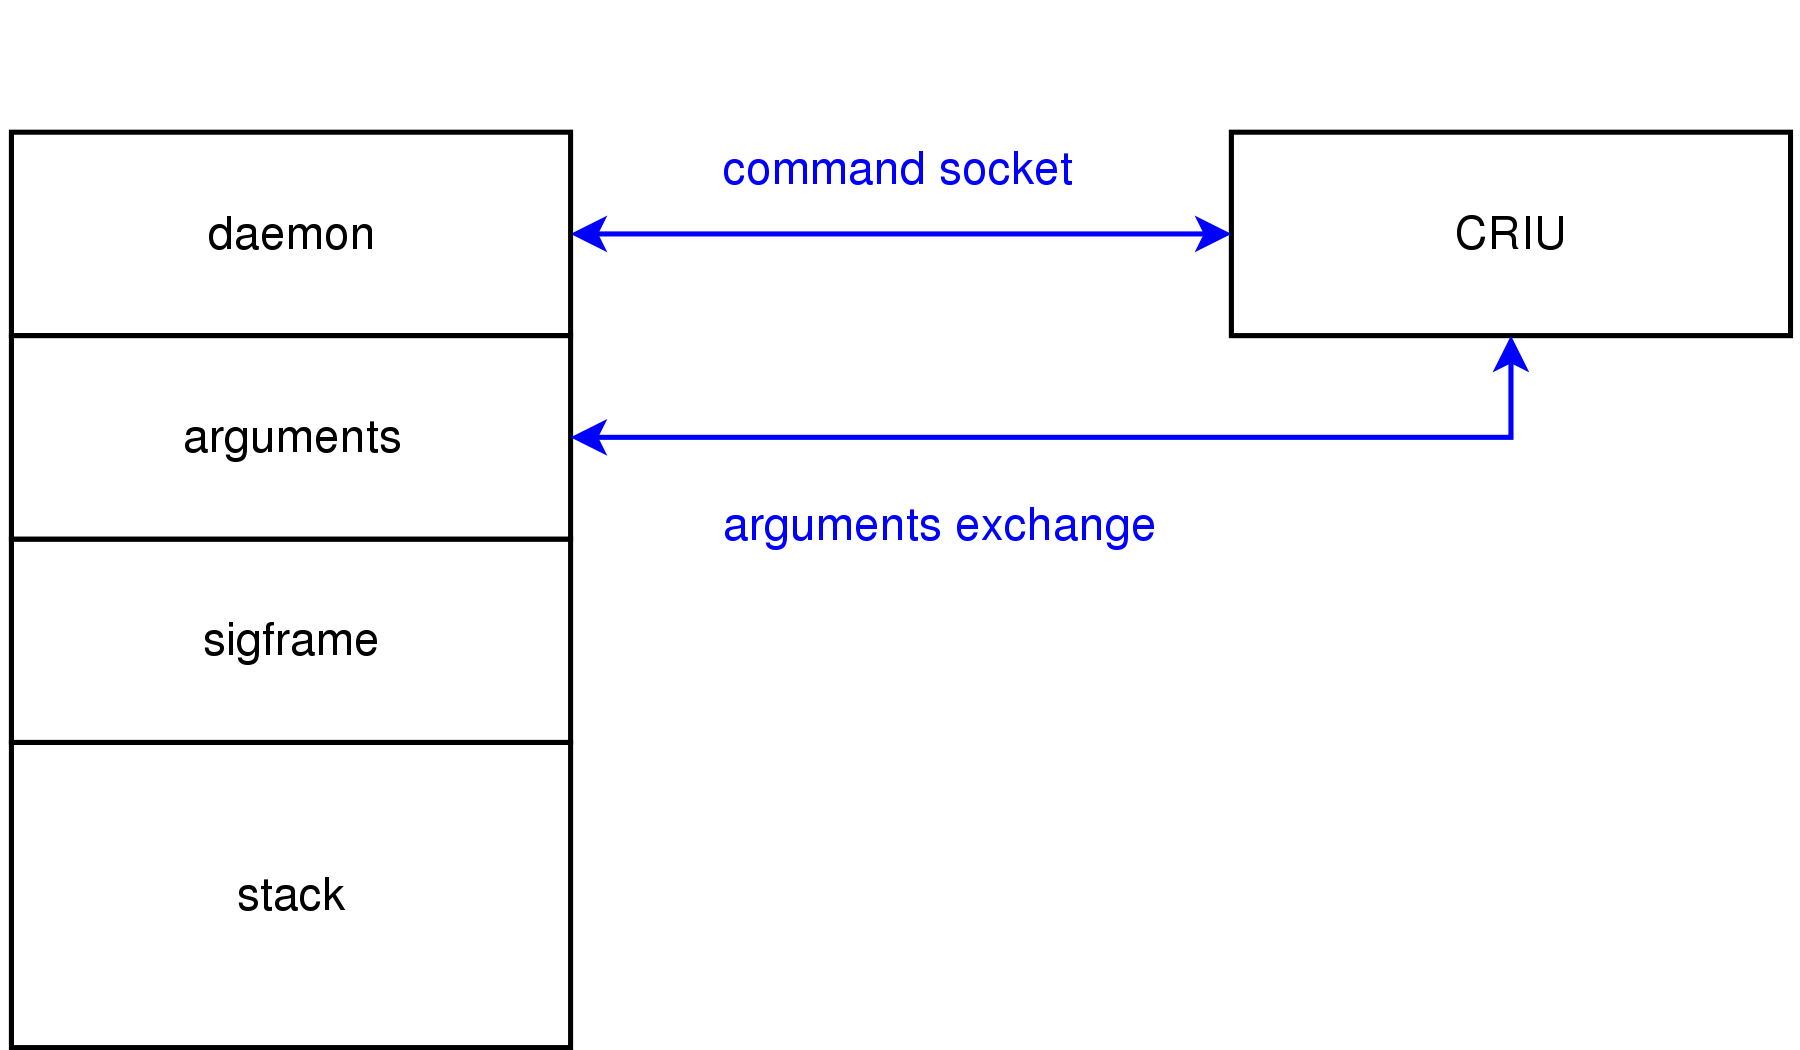
\includegraphics[width=\textwidth]{figures/criu-parasite-daemon.png}
  \end{center}
  \caption{CRIU's parasitic code acting like a daemon \cite{criu_parasite}.}
  \label{fig:parasite-daemon}
\end{figure}

In the third and last stage, after everything has been dumped, CRIU sends a command to the parasite code to finish, the parasite memory area is unmapped from dumpee, and the original instructions, together with the instruction pointer and registers are restored to the state before the parasite injection, thus \emph{curing the dumpee} \cite{criu_parasite}. Depending on the configuration, CRIU can then detach from the dumpee and unfreeze the process tree as if nothing happened or kill the whole process tree.

\subsection{Process restoration}
To restore a process, CRIU first reads all image files and finds which processes share resources. After that, CRIU starts morphing itself to the process tree it should restore by calling the \emph{fork()} system call. However, CRIU has not yet recreated all threads. In stage three, CRIU opens necessary files, prepares namespaces, changes the working and root directory, maps and fills private memory areas, creates sockets and other resources. Nevertheless, it leaves restoration of the exact memory mapping locations, timers, process credentials, and threads to the last stage \cite{criu_cr}.

CRIU has other intricate problems that must be solved in the last stage. As CRIU is morphing itself into the dumpee, it should un-map the memory belonging to CRIU and map the memory belonging to the dumpee. The first problem is that, immediately after CRIU unmaps its memory, the next instruction would be read from a memory location not belonging to the process, resulting in a segmentation fault. The second problem is that the memory mappings of the dumpee might overlap with CRIU memory. Similarly to the parasitic code for dumping, CRIU uses position-independent code referred to as the \emph{restorer context} to solve these problems. CRIU allocates a new chunk of memory that does not intersect the memory of CRIU or the memory of dumpee and puts there the data required for the restorer context and the code of the restorer itself. CRIU then \emph{jumps} to the restorer context, cleanses CRIU memory mappings and restores all the remaining resources, completing the morphing to the dumpee \cite{criu_restorer}.


\subsection{Caveats}
CRIU is not capable of checkpointing and restoring every possible Linux process. The main reason behind this is that processes can use a resource, such as a block device, which does expose its inner state. The hardware behind the block device might not even exist on the machine where restoring is triggered. This problem is usually avoided when working with containers, as containers should contain everything needed in the image. However, when checkpointing a container, CRIU also needs to dump the top file system layer of the container so that upon restoration, the restored container can see the changes made to files that were not opened at the time of checkpointing.


For the purposes of this thesis, checkpointing and restoring Jupyter Notebooks, there are two CRIU configuration options in need of explaining:

\begin{description}

    \item[tcp-close] This option ensures that sockets are restored in a closed state on restoration. This option is required for Jupyter Notebooks in the Kubernetes Cluster because a Pod created from a restored container will likely have a different IP address than the original Pod. Without this option enabled, CRIU will try to create a TCP socket with the original IP address, which will likely fail, and as a result, the whole restoration will fail.
    
    \item[file-locks] Applications like Jupyter Notebook use file locks for synchronization. Setting this option ensures that file locks are dumped and restored. CRIU does not dump the locks by default, as it does not know whether a process outside the dumpee might rely on the lock. However, in the context of containers, enabling this setting is safe.

\end{description}


\section{Checkpoint/Restore in Kubernetes and container runtimes}
\label{sec:criu:kubernetes}

Checkpointing a container is not directly possible through the Kubernetes API. Instead, checkpointing is possible only by using the Kubelet API, specifically through an HTTP request \cite{k8s_kubelet_api}:

\begin{description}
    \item[POST /checkpoint/\{namespace\}/\{pod\}/\{container\}] where namespace, pod, and container are path parameters representing the names of these objects present in the Pod manifest. Additionally, a query parameter \emph{timeout} can be provided, specifying time in seconds, after which the checkpointing will be aborted.
\end{description}
The result of the request is a \emph{tar} archive file located in the \emph{/checkpoints} directory below Kubelet's root directory containing the checkpoint of the container.

Checkpointing was introduced in 2022 with Kubernetes v1.25 as an alpha feature and had to be enabled for the Kubelet through a feature gate \emph{ContainerCheckpoint}. However, since Kubernetes v1.30, released in April 2024, checkpointing has been promoted to a beta state and is thus enabled by default.

\begin{figure}[H]
  \begin{center}
  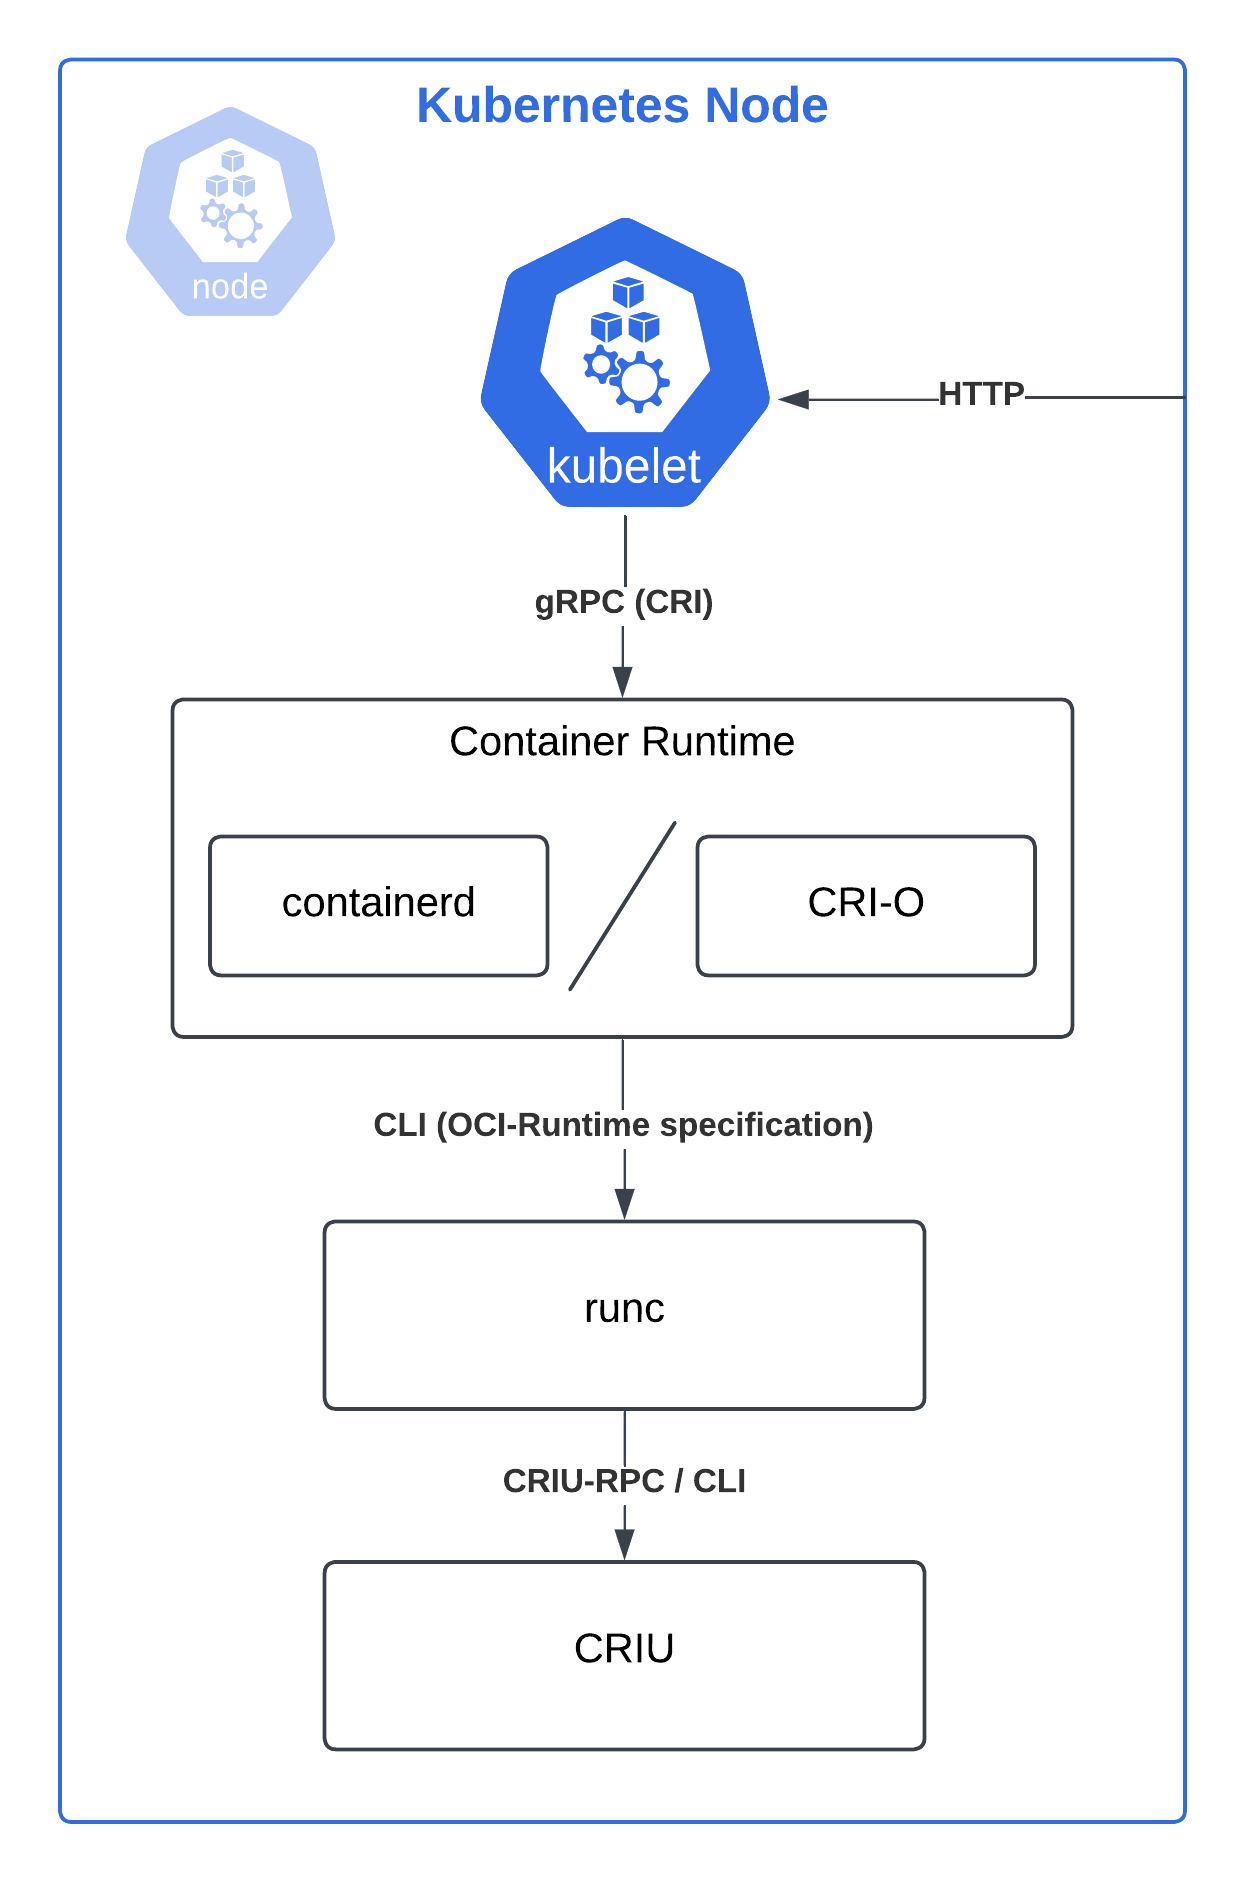
\includegraphics[width=.6\textwidth]{figures/checkpoint-callchain.png}
  \end{center}
  \caption{Call--chain for checkpointing a container in Kubernetes.}
  \label{fig:criu-calltrace}
\end{figure}

With all that said, Kubelet does not do the actual checkpointing itself. As \Cref{fig:criu-calltrace} illustrates, the kubelet will request a checkpoint from the high--level container runtime on the Node, such as containerd or CRI-O. In turn, the high--level container runtime requests checkpointing from a low--level container runtime like \emph{runc}, which finally invokes CRIU to checkpoint the container. This call--chain implies that not only Kubelet has to provide API for checkpointing, but also the high and low level container runtimes.

While the initial support for checkpointing in runc was available as early as 2015, the support for checkpointing in CRI-O and containerd can be largely accredited to Adrian Reber, who provided the implementation, invokable from kubelet, for CRI-O\footnote{\url{https://github.com/cri-o/cri-o/pull/4199}} in version v1.25.0 and containerd\footnote{\url{https://github.com/containerd/containerd/pull/6965}} in version v2.0.0.


\subsection{Restoring a container outside Kubernetes}
\label{subsec:restoring}
Conversely, restoring a container is impossible through the standard Kubernetes or kubelet API, as the Kubernetes community has yet to agree upon how such an API would look or if it even has sufficient use cases. Since Pod is the smallest deployable unit in Kubernetes, the restored container would have to be mapped to a Pod, and it needs to be clarified which component should handle this mapping, if any.

Fortunately, there is a mechanism in CRI-O and soon might be in containerd\footnote{\url{https://github.com/containerd/containerd/pull/10365}} as well, implemented by the aforementioned Adrian Reber, which allows starting a container from a container image that was created previously through checkpointing. When a container is scheduled to start, the container runtime checks the annotations of the container image. If a specific annotation is present, it triggers a restore of the container rather than a normal start. The annotations are:
\begin{description}
    \item[io.kubernetes.cri-o.annotations.checkpoint.name] for CRI-O.
    \item[org.criu.checkpoint.container.name] for containerd.
\end{description}

By providing such an image, the definition of the container in the Pod manifest is mostly ignored. Nevertheless, if the container runs in the same environment as before the checkpoint, it will continue to run as expected.


\chapter{Checkpoint/Restore of Jupyter Notebooks in Kubernetes}
The idea behind checkpoint/restore of Jupyter Notebooks is straightforward. When JupyterHub requests to stop a Notebook, either due to user's inactivity or based on user's decision, the Spawner will first checkpoint the Notebook and only afterward stop it. The next time user starts his Notebook, the Spawner, rather than spawning a regular Notebook, restores the previous checkpoint of the Notebook. Translating this idea into Kubernetes means that the KubeSpawner, the Spawner of Z2JH distribution, needs to be extended to provide checkpoint/restore capabilities. The Z2JH distribution was chosen as the more scalable of the two options provided by JupyterHub.

% Motivation and potential benefits gained by extending JupyterHub with checkpoint/restore capabilities were partly outlined in \Cref{chap:cr}. However, because JupyterHub is in control when Pods (Notebooks) are deleted, there are additional benefits. For example, Jupyter Notebooks can run in Kubernetes without a PersistentVolume and  

\section{Architecture of the prototype}
As JupyterHub is not the only application that would benefit from checkpoint/restore capabilities in Kubernetes, one of the first design decisions was to split the c/r functionality into a separate service called \emph{Checkpointer} (\Cref{chap:checkpointer}). The service was designed to be generic and oblivious to the existence of JupyterHub. It exposes HTTP API to allow any application in the cluster, possibly even outside the cluster, to request a container checkpoint, build it into a container image, and push it to a container registry.

On the other hand, the logic required to integrate JupyterHub with the Checkpointer, exists as a component called \emph{CheckpointSpawner} (\Cref{chap:checkpoint_spawner}) running within JupyterHub as a Spawner. The responsibility of CheckpointSpawner is to keep track of Notebook checkpoints and spawn a Notebook from a checkpoint.

\Cref{fig:checkpoint-highlevel} illustrates how CheckpointSpawner and Checkpointer work in unison to extend JupyterHub with checkpoint/restore capabilities. When a user authenticates and starts a Notebook for the first time, CheckpointSpawner will create a new Notebook Pod from a container image specified in the JupyterHub configuration. Once the user requests\footnote{Same logic applies if JupyterHub stops the Notebook due to user inactivity.} to stop his Notebook, CheckpointSpawner requests a checkpoint of the user's Notebook from Checkpointer, which in turn triggers the checkpointing process in the background. This asynchronous process is described more in detail in \Cref{chap:checkpoint_spawner}. The next time the Notebook is requested to start, CheckpointSpawner notices that there should be a checkpoint of the Notebook made, and it will ask Checkpointer for the container image name. Checkpointer will wait for checkpointing to finish if necessary and responds with the image name. Finally, CheckpointSpawner creates a new Pod with the checkpointed container image name.

\begin{figure}[H]
  \begin{center}
  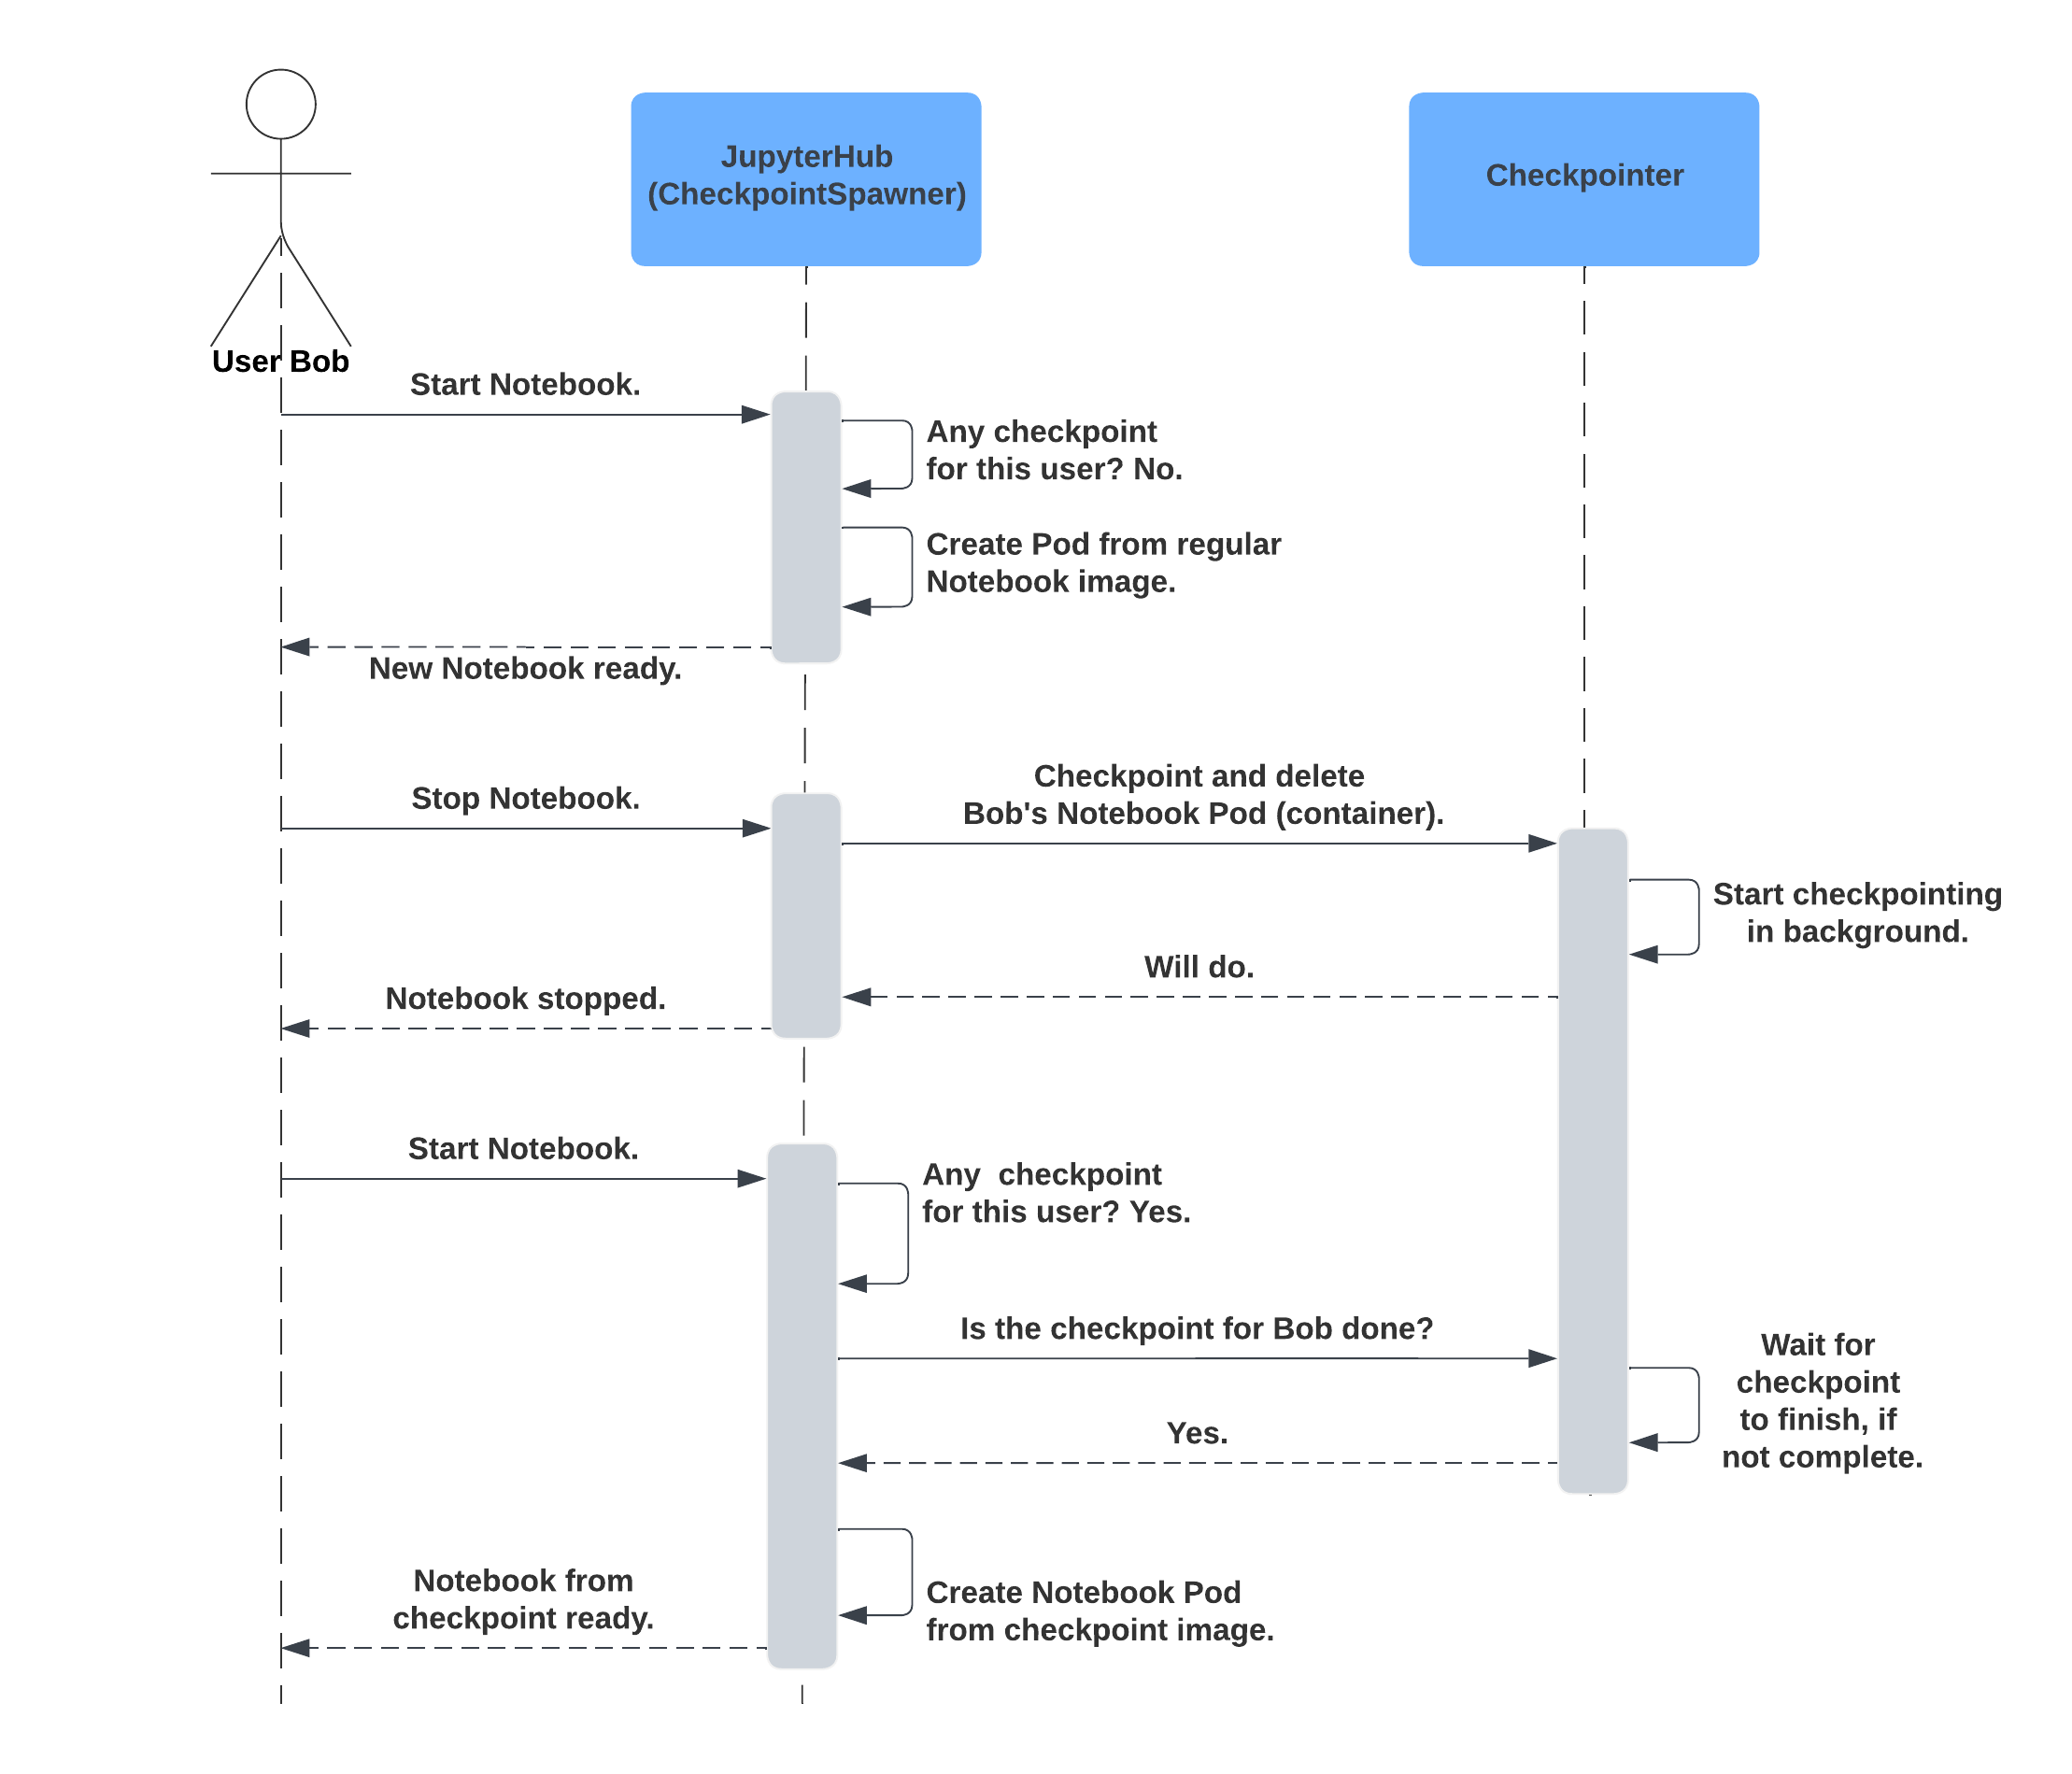
\includegraphics[width=\textwidth]{figures/checkpoint-highlevel.png}
  \end{center}
  \caption{Abstract sequence diagram of Jupyter Notebook checkpoint/restore.}
  \label{fig:checkpoint-highlevel}
\end{figure}

\subsection{Checkpoint/Restore of multi--container Notebooks}
The Z2JH JupyterHub distribution allows customizing the manifest of the Notebook Pod, which can include specifying multiple containers. These containers might be used to initialize the Notebook container or run alongside it, providing additional functionality. However, due to the increased complexity and scope of checkpointing and restoring multiple containers inside a Pod, this thesis focuses only on checkpoint/restore of the Notebook container. When CheckpointSpawner creates a Pod from a checkpointed container image, it will include the other pre--configured containers. Nevertheless, these containers start as any other regular containers, and their internal state before checkpointing will be lost. Consequently, the Pod from the restored Notebook works most reliably when it contains only the Notebook container.


\section{Runtime Environment}
\label{sec:runtime-env}
Due to the requirements for checkpoint/restore in Kubernetes, outlined in \Cref{sec:criu:kubernetes}, the prototype in this thesis was developed and tested on a \emph{manually} created and configured Kubernetes cluster hosted on CESNET MetaCentrum\footnote{\url{https://www.metacentrum.cz/en/}}. The cluster consists of one control--plane Node and one worker Node initialized through the Kubeadm tool. The Nodes communicate through a private network set up in MetaCentrum. The following list describes which versions of runtimes were used and why:

\begin{description}
    \item[Linux distribution: Ubuntu 22.04 LTS] This distribution was chosen due to experience with Ubuntu and the wide availability of Debian packages. The specific version was the latest Ubuntu release with long-term support (meanwhile, 24.04 LTS was released).
    
    \item[CRIU v3.19 built from source] Chosen as the latest stable release of CRIU. Older 3.x versions could work as well. Note that support for version 2 cgroups was introduced in v3.15.
    
    \item[Kubernetes v1.30] One of the latest versions with support ending in mid--2025. Additionally, the checkpoint API of kubelet has reached a beta state and is thus enabled by default, which shortens the required configuration.

    \item[CRI--O v1.30] This version is a natural choice as CRI-O follows the Kubernetes release cycle. Similarly to Kubernetes, starting from v1.30, CRI--O has the option \emph{enable\_criu\_support} enabled by default, shortening the required configuration.
        
    \item[containerd patched v2.0.0--rc.3] Currently, the latest stable version of containerd does not support restoring. For this reason, the prototype uses the patched version by Adrian Reber from \url{https://github.com/containerd/containerd/pull/10365}.

    \item[runc version: v1.2.0--rc.2 built from source] Relatively recent version that was tested to work with both the patched containerd as well as CRI-O. % TODO: test cgroups v2

\end{description}

The provisioning of the virtual machines was done through the user interface of OpenStack in MetaCentrum and is thus not part of this thesis. However, a shell script with commands that install and build necessary binaries and then install Kubernetes cluster is provided in \Cref{apendix}. Note that due to the unpredictability of IP addresses and hostnames and the choice of container runtime, the script should be used in a cut--and--paste manner rather than executed as a whole.



\chapter{Checkpointer}
\label{chap:checkpointer}

Checkpointer is a standalone application written in Go, designed to run as a Pod on each Node within the Kubernetes cluster. The primary purpose of Checkpointer is to checkpoint a container and build a container image that can be used to restore the container. Checkpointer exposes HTTP API to provide this functionality.

\section{Checkpointer API}
The time it takes to checkpoint a container is directly proportional to the memory usage as well as the size of the container file system. Additionally, since Checkpointer also builds and pushes a container image from this checkpoint, the time from the beginning of a request to the result might span from tens of seconds to several minutes. Applications, including JupyterHub, are generally unprepared to wait that long for a response. For this reason, the API of Checkpointer consists of two endpoints, one for requesting a checkpoint and the other for getting the result.

\subsection{Requesting a checkpoint}
To request a checkpoint, Checkpointer exposes the endpoint:
\begin{description}
  \item \texttt{[HTTP POST] /checkpoint/\{namespace\}/\{pod\}/\{container\}}
\end{description}
The endpoint mimics the Kubelet checkpoint API (\Cref{sec:criu:kubernetes}) as invoking this endpoints triggers checkpoint of a container. However, the end--result is not a tar archive on a Node, rather a container image that is pushed to remote container registry. The endpoint expects an input body in JSON format with two boolean options: \texttt{deletePod} and \texttt{async}. 

The \texttt{deletePod} option tells Checkpointer whether it should delete the Pod after checkpointing. Checkpointer will delete the Pod only if the checkpointing succeeded. More importantly, the \texttt{async} option determines if the checkpointing will happen synchronously or asynchronously. When the option is set to \texttt{false}, Checkpointer will respond to the HTTP request only after the checkpointing finished, be it successfully or not. The JSON response body can be seen on \Cref{lst:checkpoint:response} and apart from metadata includes the actual checkpointed container image name. If the checkpointing failed, as can happen if Checkpointer is misconfigured for example, the response will explain the error in plain text.

\begin{code}
\captionof{listing}{Example of checkpoint result response.}
\label{lst:checkpoint:response}
\begin{minted}{json}
{
  "containerIdentifier": {
    "namespace": "default",
    "pod": "timer-sleep",
    "container": "timer"
  },
  "beginTimestamp": 1733668372,
  "endTimestamp": 1733668440,
  "containerImageName":
  "pbaran555/kaniko-checkpointed:3440892ddc2fa56c"
}
\end{minted}
\end{code}

On the other hand, when \texttt{async} is set to \texttt{true}, Checkpointer will start the checkpointing in the background, and immediately respond to the request with a \texttt{checkpointIdentifier} string as shown on \Cref{lst:checkpoint:response:async}. The identifier can be used with the second endpoint at any time in the future to obtain the result of checkpointing.


\subsection{Result of checkpoint}
When the user requested an asynchronous checkpoint, he can obtain the result by calling:
\begin{description}
  \item \texttt{[HTTP GET] /checkpoint?checkpointIdentifier=\{...\}}
\end{description}
This endpoint expects a \texttt{checkpointIdentifier} as a query parameter with previously obtained string value. When called, the endpoint will wait until the checkpointing is finished and respond with the same result as seen on \Cref{lst:checkpoint:response}.


The asynchronous design of the API means that Checkpointer requires persistent storage. If this were not the case, restarting the Checkpointer Pod would result in the loss of all the checkpoint results accumulated during its run. To avoid such a situation, Checkpointer uses a simple file system storage, where each checkpointing result resides in a separate file in a configurable directory. The storage additionally includes an in--memory cache layer to speed up the API response time.

\begin{code}
\captionof{listing}{Example of asynchronous checkpoint response.}
\label{lst:checkpoint:response:async}
\begin{minted}{json}
{
  "checkpointIdentifier": "worker-node:3440892ddc2fa56c"
}
\end{minted}
\end{code}

\section{Running in multi-Node cluster}
Since each Kubernetes Node has an instance of Checkpointer running on it, a question arises. When a request comes to a Checkpointer on Node \emph{A}, what happens if the container to be checkpointed is running on Node \emph{B}? To be able to checkpoint container running on \emph{any} Node, Checkpointer contains a middleware called \texttt{RoutingProxy}. The role of the RoutingProxy is to intercept requests coming to a Checkpointer instance and re--route them to other Checkpointer if necessary. Re--routing in this context means that Checkpointer on Node A will serve as a reverse proxy to Checkpointer on Node B. RoutingProxy needs to decide whether the request is meant for the Checkpointer it is a part of or another and the algorithm for doing so is different depending on the type of request.

When RoutingProxy intercepts the checkpointing request (POST), it uses the Kubernetes API to determine which Node is the container to be checkpointed running on. When it finds the Node, it then looks for the IP address of the Checkpointer instance on that Node. Finally, it proxies the request to the other Checkpointer instance.

For users to get the result of checkpointing (GET) through any Checkpointer instance, the RoutingProxy relies only on the information in the checkpointIdentifier query parameter. There would be no point in including the Pod and Namespace of the checkpointed container in the request as the Pod might have already been deleted. Therefore, the checkpointIdentifier itself contains name of the Node where the checkpointing was triggered. RoutingProxy again uses the Kubernetes API to find the IP address of the targeted Checkpointer and proxies the request.

\begin{figure}[H]
  \begin{center}
  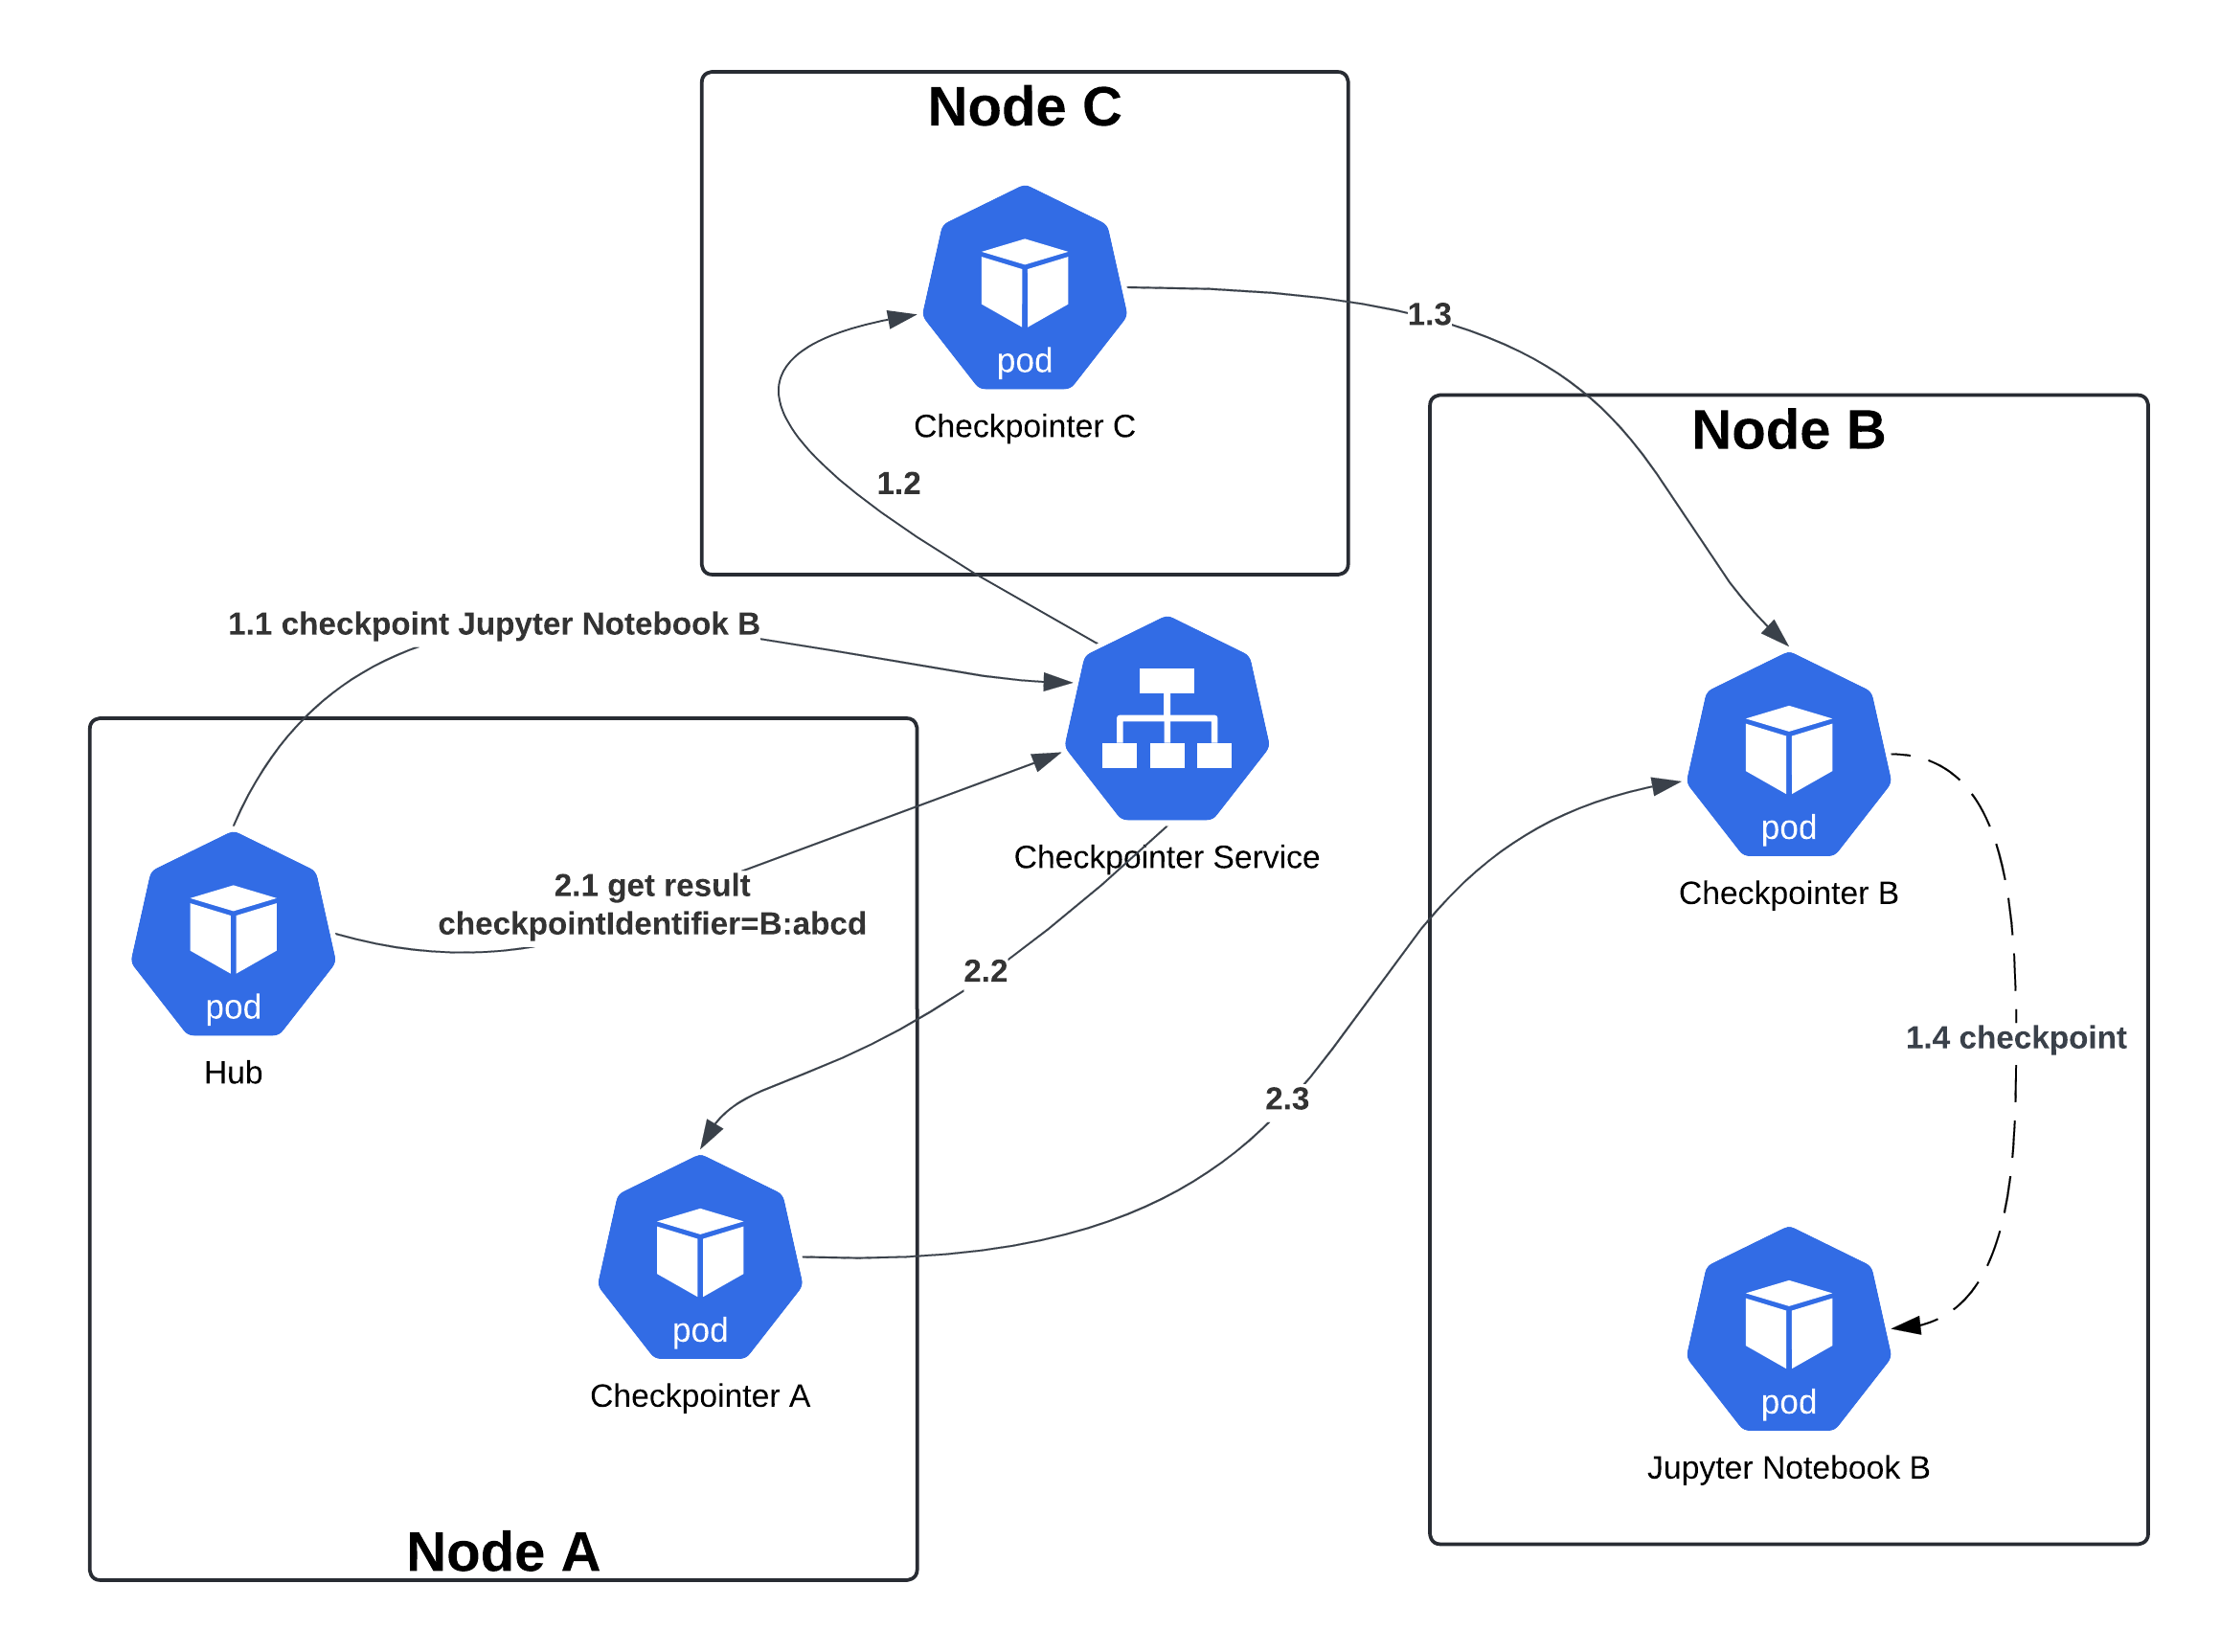
\includegraphics[width=\textwidth]{figures/multi-cluster-checkpoint.png}
  \end{center}
  \caption{Checkpointer in multi-Node cluster.}
  \label{fig:multi-cluster-checkpoint}
\end{figure}

\Cref{fig:multi-cluster-checkpoint} illustrates how requests from Hub Pod eventually reach Checkpointer B Pod. This design allows to asynchronously checkpoint and get the result of checkpointing through any Checkpointer instance. Moreover, the design does not require the Checkpointer instances to consistently synchronize whenever a new checkpointing request is received.

It should be noted that the RoutingProxy can be completely turned off, which can be useful for development purposes or when Checkpointer is running in a single-Node cluster.

\section{Checkpointer inner workings}
Checkpointing containers and creating container images in a Kubernetes cluster involves coordinating multiple processes. First, the Kubelet checkpoint API is used to create checkpoint archives, requiring Checkpointer to reach Kubelet and access the stored data. Next, the checkpointed state is used to build a container image and push it to a registry. Checkpointer avoids using tools like Docker and instead uses Kaniko, a tool for building containers within Kubernetes.


\subsection{Using Kubelet checkpoint API}
To checkpoint a container, Checkpointer makes a request to the Kubelet checkpoint API, which will result in a checkpoint archive on the file system of the Node. This approach requires Checkpointer to deal with two issues. The first issue is that Checkpointer, running \emph{within} Kubernetes cluster as a Pod, has to be able to reach Kubelet, running \emph{outside} the cluster on a Node. To be able to reach Kubelet, Checkpointer expects the IP address of the Node it is running on and the port Kubelet is listening on as environment variables. Additionally, Kubelet requires consumers of the API to authenticate using TLS certificate. Hence, Checkpointer expects this certificate together with a private key as files on the file system (see \Cref{sec:manifests}). The location of these files can be configured through environment variables as well. The second issue is that Checkpointer has to be able to access the checkpoint archives made by Kubelet. For that, the Checkpointer Pod is configured with a volume mount pointing to the directory on the host, where Kubelet stores the archives.

\subsection{Building container images with Kaniko}
\label{sec:kaniko-strategies}
After checkpointing a container, Checkpointer needs to create a container image and push it to a remote registry. However, building a container image \emph{from within a container} with tools like Docker would require the Checkpointer container to run as privileged, which is not ideal for production environments as it imposes a security risk. Therefore, Checkpointer uses an open--source tool called \emph{Kaniko}\footnote{\url{https://github.com/GoogleContainerTools/kaniko}}, designed to run as a container within Kubernetes and build containers in user--space.

Checkpointer creates a Kaniko Pod to build and push the checkpoint container image. To build a container image, Kaniko requires a \emph{build context}, which includes a Dockerfile and all the files that should be included in the container image. Additionally, Kaniko must know where to push the container image and have the required credentials. When Checkpointer creates the Kaniko Pod manifest, it includes the name of the checkpoint container image name in the command line arguments of the Kaniko container. To provide the registry credentials, Checkpointer includes in the manifest a volume mount for a Kubernetes Secret containing the credentials. The creation of this Secret is part of the deployment steps, and Checkpointer assumes that the Secret already exists but provides a configuration option to specify its name.

\begin{figure}[H]
  \begin{center}
  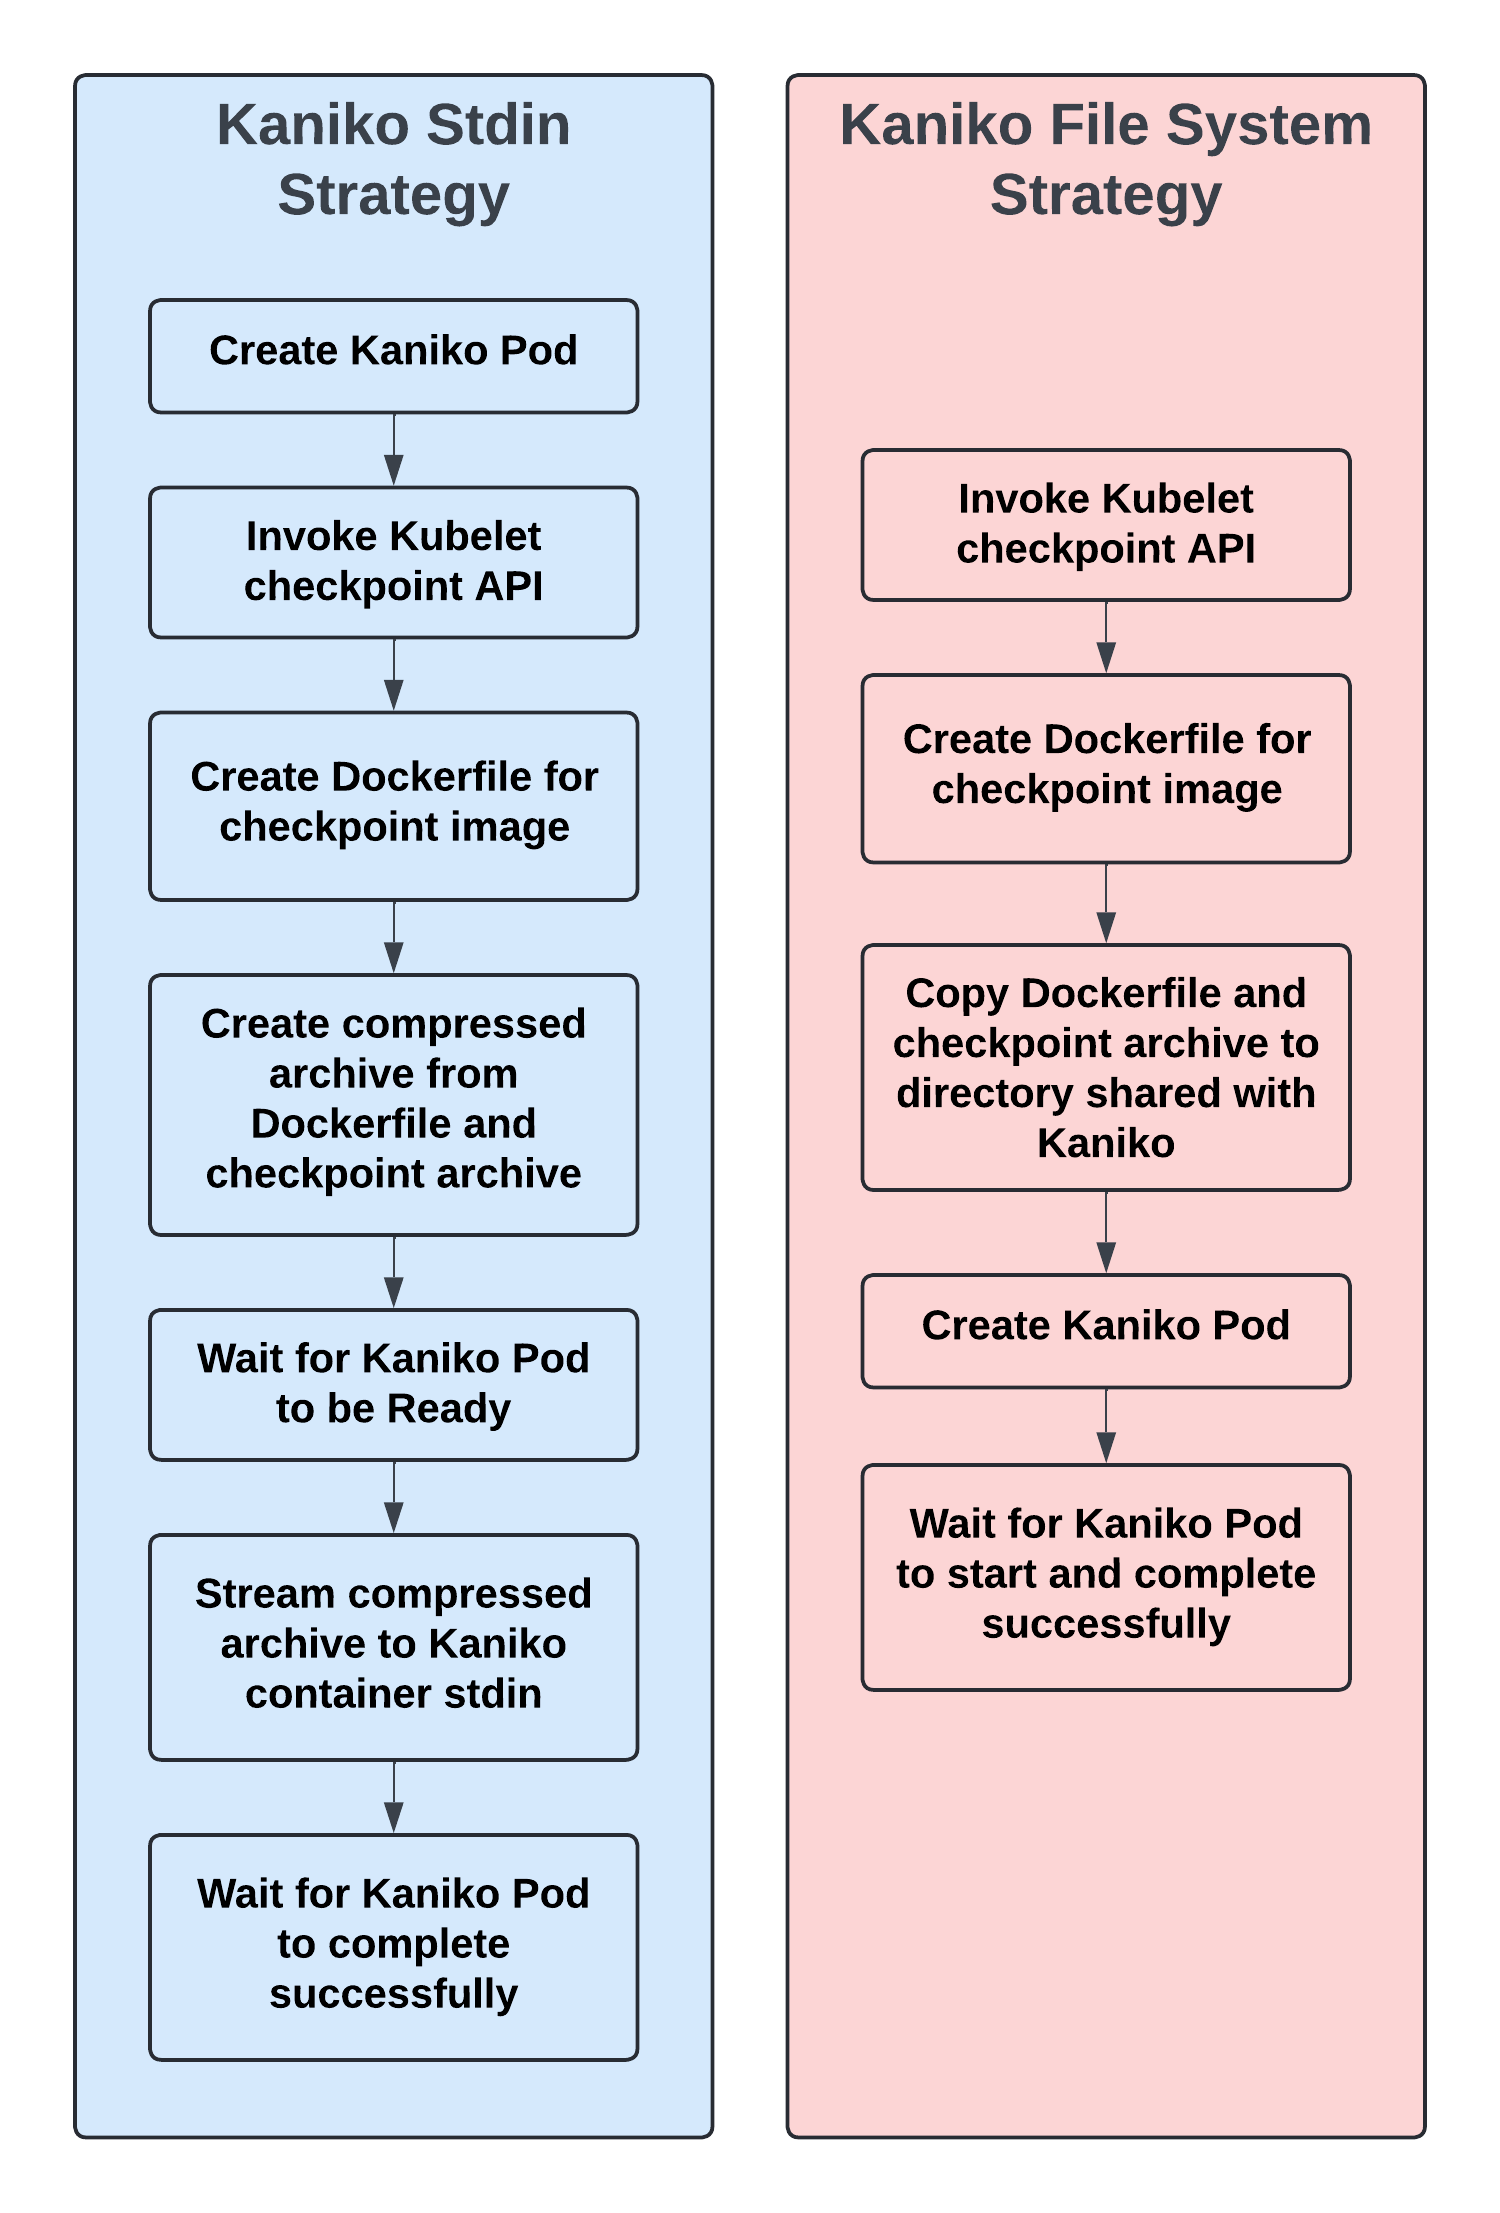
\includegraphics[width=.5\textwidth]{figures/kaniko-strategies.png}
  \end{center}
  \caption{Comparison of Kaniko strategies.}
  \label{fig:kaniko-strategies}
\end{figure}

Providing the build context for Kaniko is a more complicated process. Kaniko can accept the build context through various methods, but only two are relevant to this thesis. The first way is to mount a directory containing the build context into the Kaniko Pod. The second way is to write the whole build context as a compressed archive to the standard input (stdin) of the Kaniko container. Checkpointer can be configured to use either of the two strategies, but it affects the algorithm Checkpointer uses. The differences between the two strategies can be observed on \Cref{fig:kaniko-strategies}.


By default, Checkpointer uses the \emph{Stdin strategy}. Consequently, Checkpointer needs to archive and compress the build context. Moreover, Checkpointer needs RBAC permissions to attach to a Pod (see \Cref{sec:manifests}). Although the File System strategy looks simpler, the Stdin strategy offers an advantage over the other due to how long it takes for Kaniko Pod to start. Using the Stdin strategy, Checkpointer can create the Kaniko Pod before calling the Kubelet checkpoint API, which means that while Kaniko Pod is initializing, Kubelet can create the checkpoint archive. With the second strategy, at the start of Kaniko, the build context must already be present on Kaniko's file system, which means that Checkpointer must create the Kaniko Pod only after Kubelet has finished creating the checkpoint archive. In this case, non--trivial amount of time is wasted waiting for Kaniko Pod to start.

\subsection{Base image of checkpoint container image}
\label{sec:base-image}
Using Kaniko for container building comes with one pitfall. As \Cref{subsec:restoring} explained, the container image needs to have the appropriate annotation for container runtime to trigger a container restore. However, at the time of writing, Kaniko does not allow the configuration of annotations for the images it builds. As a solution to this problem, this thesis provides a base image \texttt{pbaran555/checkpoint-base:latest} created \texttt{FROM scratch} and annotated with annotations required for both containerd and CRI-O. Checkpointer will use this image as the base image for all checkpoint container images. Checkpointer can be configured (\Cref{sec:checkpointer:configuration}) to use a different base image, provided it is accessible publicly or using the credentials that Kaniko consumes. In this case, users need to make sure the base image is correctly annotated for their container runtime.


\section{Kubernetes manifests}
\label{sec:manifests}
For Checkpointer to run in Kubernetes without any issues, it needs to be deployed with Kubernetes resources (manifests) defined in \texttt{k8s-manifests} directory of \Cref{apendix}. The following list provides a summary of what they are and why they are needed:

\begin{description}
    
    \item[DaemonSet] Deploying Checkpointer as DaemonSet allows it to run automatically on every Node. If a new Node joins the cluster, Kubernetes will create a new Checkpointer Pod on that Node and recreate a Pod in case the Pod is deleted from a Node. The DaemonSet contains two sets of important configuration settings: the environment variables and the volume mounts.

    The environment variables like \texttt{CHECKPOINTER\_NODE} or \\ \texttt{CHECKPOINTER\_NODE\_IP} have to be set by Kubernetes for Checkpointer to run correctly in a multi-Node cluster. On the other hand, Checkpointer requires specific volume mounts, whose configuration depends on the Kubernetes installation. The \\ \texttt{checkpoints-tar-dir} mount allows Checkpointer to access the tar archives (checkpoints) created by the Kubelet. Mount called \texttt{build-contexts-dir} is for temporary transfer of build contexts to Kaniko and is only required in case Checkpointer is configured to use the Kaniko file system strategy. Lastly, \\
    \texttt{kubelet-tls-secret} mount loads a TLS certificate and key required for Checkpointer to authenticate to Kubelet.
    
    \item[ConfigMap] Used for Checkpointer configuration. Checkpointer consumes the key--value pairs from ConfigMap as environment variables.
    
    \item[Secret] The Secret of type \texttt{dockerconfigjson} is not directly consumed by the Checkpointer itself. The credentials contained by the Secret are consumed by the Kaniko Pod that Checkpointer creates to push the checkpoint image to a remote container registry.
    
    Furthermore, the \texttt{tls} Secret is required by the Checkpointer to authenticate itself to Kubelet when invoking Kubelet API. As previously mentioned, the Secret is mounted into Checkpointer as \texttt{kubelet-tls-secret}.
    
    \item[ClusterRoleBinding, ClusterRole, and ServiceAccount]
    Using the Kubernetes API to list or delete Pods requires RBAC permissions. Checkpointer needs to be able to get, list, delete, and attach to Pods across cluster. Thus, three resources need to be created: ClusterRole with the specified permissions, ServiceAccount, which the Checkpointer attaches (in the DeamonSet), and lastly ClusterRoleBinding, which binds the ServiceAccount to the ClusterRole.
    
    \item[Service] This Service of type \texttt{ClusterIP} allows JupyterHub to connect to Checkpointer from inside the cluster. This Service type can be customized, for example, to expose Checkpointer API outside the cluster.

\end{description}

\section{Configuration options}
\label{sec:checkpointer:configuration}
Because Checkpointer runs in Kubernetes, it was designed to be configured through environment variables so that all the configuration options can be centralized in a Kubernetes ConfigMap. The configuration can be divided into three categories: required, configuration related to Kubelet, and generic.

The environment variables below are required, and Checkpointer will terminate itself if they are not present at the startup. However, the Namespace, Node, and IP address should be set by Kubernetes through the mapping defined in the DaemonSet. The user needs only to define the image repository where Checkpointer will push the checkpoint images. The repository should be accessible using the credentials in the \texttt{dockerconfigjson} Secret.

\begin{description}
    \item[\texttt{CHECKPOINT\_IMAGE\_PREFIX}] The container registry and repository that Checkpointer will push checkpoint images to, such as \\ \texttt{quay.io/pbaran/checkpointed}.
    \item[\texttt{CHECKPOINTER\_NAMESPACE}] Kubernetes Namespace that Checkpointer is running in.
    \item[\texttt{CHECKPOINTER\_NODE}] Name of the Node that Checkpointer is running on.
    \item[\texttt{CHECKPOINTER\_NODE\_IP}] IP address of the Node that Checkpointer is running on.
\end{description}


The variables below should be set when Kubelet is installed using non--default options or when customizing the DaemonSet. All the options have a default value pre--configured. However, the private key's location and certificate must match the mounting point defined in the DaemonSet.
\begin{description}
    \item[\texttt{KUBELET\_PORT}] Port that Kubelet listens on.
    \item[\texttt{KUBELET\_CERT\_FILE}] File path within the Checkpointer to the TLS certificate used to authenticate Kubelet.
    \item[\texttt{KUBELET\_KEY\_FILE}] File path within the Checkpointer to the private key used to authenticate Kubelet.
    \item[\texttt{KUBELET\_ALLOW\_INSECURE}] If set to \texttt{true}, Checkpointer will not verify Kubelet TLS certificate. This option is useful if Kubelet uses a self--signed certificate.
\end{description}

The last set of environment variables influences some of the inner workings of Checkpointer. All of these have a reasonable default value pre--configured.
\begin{description}
    \item[\texttt{CHECKPOINT\_BASE\_IMAGE}] Image used as a base for all checkpoint container images as described in \Cref{sec:base-image}.
    \item[\texttt{KANIKO\_SECRET\_NAME}] Name of the Kubernetes Secret with credentials for a remote container registry. The Secret has to exist in the same Namespace as Checkpointer.
    \item[\texttt{KANIKO\_TIMEOUT}] Time in seconds, after which Checkpointer will timeout waiting for Kaniko Pod to reach a certain state.
    \item[\texttt{USE\_KANIKO\_FS}] If set to \texttt{true}, Checkpointer will use the \texttt{Kaniko File System strategy} for checkpointing as described in \Cref{sec:kaniko-strategies}.
    \item[\texttt{STORAGE\_BASE\_PATH}] Directory where Checkpointer will store checkpoint results needed for its asynchronous API.
    \item[\texttt{DISABLE\_ROUTE\_FORWARD}] If set to \texttt{true}, the \texttt{RoutingProxy} will be disabled. The setting should only be used in a single--Node cluster or for development purposes.
     \item[\texttt{ENVIRONMENT}] If set to \texttt{prod}, Checkpointer will run in Production mode. By default, Checkpointer runs in Development mode. Currently, the only differences between the modes are the log level and format.
\end{description}


\chapter{CheckpointSpawner}
\label{chap:checkpoint_spawner}

CheckpointSpawner is a Python class extending KubeSpawner, the Spawner of the Z2JH JupyterHub distribution. CheckpointSpawner is not a standalone application; instead, it is implemented to run as a Spawner within the Hub component of JupyterHub. CheckpointSpawner builds on the functionality provided by KubeSpawner and adds the capabilities to checkpoint and restore Jupyter Notebook by invoking Checkpointer API. 

JupyterHub, specifically the Hub process that CheckpointSpawner runs a part of, is built upon an asynchronous Python web framework called Tornado\footnote{\url{https://www.tornadoweb.org/en/stable/}}. Tornado, and thus Hub, runs as a single-threaded non--blocking event loop and utilizes the \texttt{async/await} syntax for coroutines. JupyterHub's Spawner interface (see \Cref{sec:spawner}) defines the \texttt{start}, \texttt{stop}, and \texttt{poll} methods as coroutines. For CheckpointSpawner, this means that the HTTP client used to call Checkpointer API must also be asynchronous. Otherwise, it would risk blocking Hub's event loop and making the whole JupyterHub unresponsive.

Hub creates a new instance of the CheckpointSpawner class for each authenticated user. As discussed in \Cref{sec:spawner}, Hub can persist the internal state of Spawners through the \texttt{get\_state()} and \texttt{load\_state()} methods. Therefore, by implementing these methods, each CheckpointSpawner instance keeps track of that user's checkpointed Notebooks.


\section{Checkpointing a Notebook}
According to JupyterHub documentation, the \texttt{stop()} method should return after the Notebook is completely stopped. Indeed, the first iteration of CheckpointSpawner did not use the asynchronous API of Checkpointer (it did not exist yet). Initially, CheckpointSpawner would wait until the whole checkpoint was done and only then returned. The problem with this approach was that Hub and JupyterHub UI are not designed to wait tens of seconds to a few minutes for the Notebook to stop. Hub does have an internal configuration parameter called \texttt{slow\_stop\_timeout}, and increasing this parameter might prevent timeout errors. However, JupyterHub UI does not handle long waiting times well, regardless of the timeout parameter. Consequently, the asynchronous API of Checkpointer was developed.

When Hub calls the \texttt{stop()} Spawner method, it can do so with a boolean parameter called \texttt{now}. If this parameter is set to \texttt{true}, Hub wants to delete the Notebook as soon as possible, usually as a cleanup due to some error. In this case, CheckpointSpawner delegates stopping the Notebook to KubeSpawner, its parent class.
KubeSpawner stops the Notebook by deleting the Notebook Pod, as discussed in \Cref{sec:kubespawner}.
It is when Hub calls the method with the value set to \texttt{false} that CheckpointSpawner asynchronously requests a checkpoint from Checkpointer, stores the \texttt{checkpointIdentifier} in its internal state, and immediately \texttt{returns}.

This design's significant benefit is that the user does not have to wait for the checkpointing to finish. However, there is a hidden challenge in this approach. What happens when the user wants to start his Notebook immediately after stopping it? In the \texttt{start()} method, through its internal state, CheckpointSpawner checks whether there should be an ongoing checkpoint. If there is not, it simply delegates the spawning of the Notebook to KubeSpawner. More importantly, if there should be a checkpoint, CheckpointSpawner requests Checkpointer to get the result. This request is indeed blocking\footnote{Not in the sense of blocking the Tornado event loop.} and might take several minutes. Luckily, Hub and JupyterHub UI expect spawning to take several minutes and even provide a configuration setting \texttt{start\_timeout} to customize the timeout. Therefore, CheckpointSpawner waits for the checkpoint to complete and, after, delegates the creation of the Notebook Pod to KubeSpawner.

\section{Restoring a Notebook}
Restoring a Notebook means the Notebook Pod will use a checkpoint container image instead of a standard one. As mentioned, CheckpointSpawner delegates spawning of the Notebook Pod when there is no checkpoint of the Notebook yet. When the checkpoint image is ready, CheckpointSpawner will utilize the \texttt{modify\_pod\_hook} property of KubeSpawner. This property can be set to point to a function that will modify the Pod manifest of the Notebook. By setting this property, CheckpointSpawner does not have to rewrite the whole \texttt{start()} method from scratch but can make use of the inherited KubeSpawner functionality.


\section{Preserving Notebook credentials}
\Cref{subsec:jupyterhub:authenticator} discussed how JupyterHub can be configured with different types of Authenticators to authenticate users. However, when JupyterHub spawns a Notebook, there is one more completely separate authentication\footnote{It could be debated if it is not, in fact, an authorization process. However, that is irrelevant to this thesis.} process happening. In this process, the Notebook acts as an OAuth client, and the JupyterHub acts as an OAuth service provider. When a user connects to a Notebook, he might not even notice the OAuth flow, apart from some browser redirections. However, in reality, the user is taken through a whole OAuth \emph{authorization code flow}. The specific details of the flow are unimportant; nevertheless, at the last step of the flow, Jupyter Notebook requests an OAuth token from JupyterHub in exchange for a temporary \texttt{code} it previously obtained. Jupyter Notebook must include its \texttt{client secret} in this request. Jupyter Notebook obtains the client secret value from JupyterHub as \texttt{JUPYTERHUB\_API\_TOKEN} environment variable, which presents a challenge for CheckpointSpawner.

The creation of the secret is not part of the Spawner but an internal process of Hub. Whenever Hub instructs Spawner to spawn a Notebook, it generates a new secret value and stores it in a database. This does not pose a problem when Spawner spawns a new Notebook Pod, as it will include the newly generated secret in the environment variables. However, when CheckpointSpawner creates a Notebook Pod from a checkpoint, the Pod knows only the old client secret. Thus, the OAuth flow fails, and the user is unable to access his Notebook.

CheckpointSpawner deals with this problem in two ways. It sets a \texttt{will\_resume} Spawner property to \texttt{true}, which ensures that Hub does not delete the secret from the database. However, a new secret value is still generated in memory; thus, in the \texttt{start()} method, CheckpointSpawner has to overwrite the value with the very first client secret it saved as \texttt{initial\_api\_token} as part of its internal state. The result is that every time CheckpointSpawner spawns a checkpointed Notebook, the Notebook can use the first client secret in the OAuth flow.


\section{Using CheckpointSpawner within Z2JH}
To use CheckpointSpawner as a JupyterHub Spawner, the CheckpointSpawner class needs to be configured in \texttt{jupyterhub\_config.py} as discussed in \Cref{subsec:jupyterhub:configuration}. However, the Z2JH distribution cannot be configured through this file. As mentioned in \Cref{sec:z2jh}, Z2JH is deployed using Helm charts and configured through the \texttt{config.yaml} file in YAML format. This thesis builds on the version 4.0.0 chart, which can be found on \url{https://hub.jupyter.org/helm-chart/}. Configuring CheckpointSpawner as the Spawner involves changing two settings in the values file.

First of all the \texttt{spawner\_class} property needs to reference CheckpointSpawner through its wheel package as can be seen on \Cref{lst:z2jh:values}. However, the default Hub container image used in the Helm chart does not have access to the code of CheckpointSpawner. Therefore, a Python wheel package containing CheckpointSpawner has to be built first, and from it, a new Hub container image that imports the package. After the image is built and pushed to a container registry it can be used withing Z2JH by setting the \texttt{image} property in values file as in \Cref{lst:z2jh:values}.


\begin{code}
\captionof{listing}{Configuring Z2JH to use CheckpointSpawner.}
\label{lst:z2jh:values}
\begin{minted}{yaml}
hub:
  image:
    name: "pbaran555/hub-checkpoint-spawner"
    tag: "0.0.1"
  config:
    JupyterHub:
      spawner_class: 
        "checkpointer-spawner.CheckpointSpawner"
\end{minted}
\end{code}




\chapter{Future work}
While working on the implementation of the prototype presented in this thesis, some areas of the prototype had to be intentionally unaddressed due to the additional complexity and scope they would bring. These can be categorized into three areas: efficiency, security, and usability.

This thesis does not address the disk space occupied by checkpointed container images on the registry and Nodes. Since the checkpoint image includes the entire file system and memory, and the images do not support layer sharing, they consume significant disk space and require regular pruning.

Prototype presented in this thesis was developed with a strong emphasis on security. Checkpointer utilizes Kaniko to build checkpoint container images, removing the need for the Checkpointer container to run with privileged access. Default configuration options were chosen to be secure, requiring users to opt for less secure settings if desired explicitly. However, securing the Checkpointer HTTP API is not addressed in this work due to two key considerations: securing the HTTP API is relatively simple compared to the complexity of implementing checkpoint/restore functionality, making it appropriate for future work, and addressing it at this stage would unnecessarily complicate the development process and cluster setup.

One of the initial design ideas for Checkpointer was to make it into a Kubernetes Operator. Checkpointer, in its current state, does resemble an Operator. It runs natively in Kubernetes and uses the Kubernetes API to accomplish its tasks. However, in the end, the design choice for an HTTP API won, mainly due to the added complexity Kubernetes Custom Resources would impose on JupyterHub. The Spawner would have to be able to create Custom Resources and watch for changes in their status. These operations would require RBAC permissions, and the whole cluster setup would be even more complicated than it already is. Nevertheless, with more applications integrating with Checkpointer and more use--cases emerging as a result, it might prove beneficial to have Checkpointer running as an Operator.




\chapter{Conclusion}
TODO: approx 1 page

\printbibliography[heading=bibintoc] %% Print the bibliography.



\appendix %% Start the appendices.
\chapter{Contents of the Archive}
\label{apendix}

1. Creating Kubernetes Cluster as described in \Cref{sec:runtime-env}.

2. Creating Kubernetes TLS Secret with certificate and private key for authentication to Kubelet, and dockerconfigjson Secret with credentials to container registry.

3. Building Checkpointer image with Docker.

4. Building CheckpointSpawner package and Hub container image using importing package.

5. Deploying Checkpointer, with environment variable pointing to a remote container registry.

6. Deploying Z2JH Helm charts with overridden config.yaml.

\end{document}
